% Options for packages loaded elsewhere
\PassOptionsToPackage{unicode}{hyperref}
\PassOptionsToPackage{hyphens}{url}
%
\documentclass[
]{article}
\usepackage{amsmath,amssymb}
\usepackage{lmodern}
\usepackage{iftex}
\ifPDFTeX
  \usepackage[T1]{fontenc}
  \usepackage[utf8]{inputenc}
  \usepackage{textcomp} % provide euro and other symbols
\else % if luatex or xetex
  \usepackage{unicode-math}
  \defaultfontfeatures{Scale=MatchLowercase}
  \defaultfontfeatures[\rmfamily]{Ligatures=TeX,Scale=1}
\fi
% Use upquote if available, for straight quotes in verbatim environments
\IfFileExists{upquote.sty}{\usepackage{upquote}}{}
\IfFileExists{microtype.sty}{% use microtype if available
  \usepackage[]{microtype}
  \UseMicrotypeSet[protrusion]{basicmath} % disable protrusion for tt fonts
}{}
\makeatletter
\@ifundefined{KOMAClassName}{% if non-KOMA class
  \IfFileExists{parskip.sty}{%
    \usepackage{parskip}
  }{% else
    \setlength{\parindent}{0pt}
    \setlength{\parskip}{6pt plus 2pt minus 1pt}}
}{% if KOMA class
  \KOMAoptions{parskip=half}}
\makeatother
\usepackage{xcolor}
\IfFileExists{xurl.sty}{\usepackage{xurl}}{} % add URL line breaks if available
\IfFileExists{bookmark.sty}{\usepackage{bookmark}}{\usepackage{hyperref}}
\hypersetup{
  pdftitle={Tratamiento de valores perdidos con R},
  pdfauthor={Evelyn Gutierrez; Vilma Romero},
  hidelinks,
  pdfcreator={LaTeX via pandoc}}
\urlstyle{same} % disable monospaced font for URLs
\usepackage[margin=1in]{geometry}
\usepackage{color}
\usepackage{fancyvrb}
\newcommand{\VerbBar}{|}
\newcommand{\VERB}{\Verb[commandchars=\\\{\}]}
\DefineVerbatimEnvironment{Highlighting}{Verbatim}{commandchars=\\\{\}}
% Add ',fontsize=\small' for more characters per line
\usepackage{framed}
\definecolor{shadecolor}{RGB}{248,248,248}
\newenvironment{Shaded}{\begin{snugshade}}{\end{snugshade}}
\newcommand{\AlertTok}[1]{\textcolor[rgb]{0.94,0.16,0.16}{#1}}
\newcommand{\AnnotationTok}[1]{\textcolor[rgb]{0.56,0.35,0.01}{\textbf{\textit{#1}}}}
\newcommand{\AttributeTok}[1]{\textcolor[rgb]{0.77,0.63,0.00}{#1}}
\newcommand{\BaseNTok}[1]{\textcolor[rgb]{0.00,0.00,0.81}{#1}}
\newcommand{\BuiltInTok}[1]{#1}
\newcommand{\CharTok}[1]{\textcolor[rgb]{0.31,0.60,0.02}{#1}}
\newcommand{\CommentTok}[1]{\textcolor[rgb]{0.56,0.35,0.01}{\textit{#1}}}
\newcommand{\CommentVarTok}[1]{\textcolor[rgb]{0.56,0.35,0.01}{\textbf{\textit{#1}}}}
\newcommand{\ConstantTok}[1]{\textcolor[rgb]{0.00,0.00,0.00}{#1}}
\newcommand{\ControlFlowTok}[1]{\textcolor[rgb]{0.13,0.29,0.53}{\textbf{#1}}}
\newcommand{\DataTypeTok}[1]{\textcolor[rgb]{0.13,0.29,0.53}{#1}}
\newcommand{\DecValTok}[1]{\textcolor[rgb]{0.00,0.00,0.81}{#1}}
\newcommand{\DocumentationTok}[1]{\textcolor[rgb]{0.56,0.35,0.01}{\textbf{\textit{#1}}}}
\newcommand{\ErrorTok}[1]{\textcolor[rgb]{0.64,0.00,0.00}{\textbf{#1}}}
\newcommand{\ExtensionTok}[1]{#1}
\newcommand{\FloatTok}[1]{\textcolor[rgb]{0.00,0.00,0.81}{#1}}
\newcommand{\FunctionTok}[1]{\textcolor[rgb]{0.00,0.00,0.00}{#1}}
\newcommand{\ImportTok}[1]{#1}
\newcommand{\InformationTok}[1]{\textcolor[rgb]{0.56,0.35,0.01}{\textbf{\textit{#1}}}}
\newcommand{\KeywordTok}[1]{\textcolor[rgb]{0.13,0.29,0.53}{\textbf{#1}}}
\newcommand{\NormalTok}[1]{#1}
\newcommand{\OperatorTok}[1]{\textcolor[rgb]{0.81,0.36,0.00}{\textbf{#1}}}
\newcommand{\OtherTok}[1]{\textcolor[rgb]{0.56,0.35,0.01}{#1}}
\newcommand{\PreprocessorTok}[1]{\textcolor[rgb]{0.56,0.35,0.01}{\textit{#1}}}
\newcommand{\RegionMarkerTok}[1]{#1}
\newcommand{\SpecialCharTok}[1]{\textcolor[rgb]{0.00,0.00,0.00}{#1}}
\newcommand{\SpecialStringTok}[1]{\textcolor[rgb]{0.31,0.60,0.02}{#1}}
\newcommand{\StringTok}[1]{\textcolor[rgb]{0.31,0.60,0.02}{#1}}
\newcommand{\VariableTok}[1]{\textcolor[rgb]{0.00,0.00,0.00}{#1}}
\newcommand{\VerbatimStringTok}[1]{\textcolor[rgb]{0.31,0.60,0.02}{#1}}
\newcommand{\WarningTok}[1]{\textcolor[rgb]{0.56,0.35,0.01}{\textbf{\textit{#1}}}}
\usepackage{graphicx}
\makeatletter
\def\maxwidth{\ifdim\Gin@nat@width>\linewidth\linewidth\else\Gin@nat@width\fi}
\def\maxheight{\ifdim\Gin@nat@height>\textheight\textheight\else\Gin@nat@height\fi}
\makeatother
% Scale images if necessary, so that they will not overflow the page
% margins by default, and it is still possible to overwrite the defaults
% using explicit options in \includegraphics[width, height, ...]{}
\setkeys{Gin}{width=\maxwidth,height=\maxheight,keepaspectratio}
% Set default figure placement to htbp
\makeatletter
\def\fps@figure{htbp}
\makeatother
\setlength{\emergencystretch}{3em} % prevent overfull lines
\providecommand{\tightlist}{%
  \setlength{\itemsep}{0pt}\setlength{\parskip}{0pt}}
\setcounter{secnumdepth}{5}
\ifLuaTeX
  \usepackage{selnolig}  % disable illegal ligatures
\fi

\title{Tratamiento de valores perdidos con R}
\author{Evelyn Gutierrez\footnote{\href{mailto:egutierreza@pucp.edu.pe}{\nolinkurl{egutierreza@pucp.edu.pe}}} \and Vilma
Romero\footnote{\href{mailto:vromero@uni.pe}{\nolinkurl{vromero@uni.pe}}}}
\date{September, 2021}

\begin{document}
\maketitle

{
\setcounter{tocdepth}{2}
\tableofcontents
}
\hypertarget{introducciuxf3n.}{%
\section{Introducción.}\label{introducciuxf3n.}}

\hypertarget{laboratorio-en-r.}{%
\section{Laboratorio en R.}\label{laboratorio-en-r.}}

En esta sesión, realizaremos la imputación de datos perdidos utilizando
técnicas básicas y por vecinos más cercanos.

Requerimos instalar los siguientes paquetes:

\begin{itemize}
\tightlist
\item
  \texttt{Hmisc}
\item
  \texttt{VIM}
\item
  \texttt{mice}
\item
  \texttt{DMwR}
\end{itemize}

Para \texttt{DMwR}, utilizar:
\texttt{remotes::install\_github("cran/DMwR")}

\hypertarget{exploraciuxf3n-de-valores-perdidos.}{%
\section{Exploración de valores
perdidos.}\label{exploraciuxf3n-de-valores-perdidos.}}

\hypertarget{exploraciuxf3n-buxe1sica.}{%
\subsection{Exploración básica.}\label{exploraciuxf3n-buxe1sica.}}

\textbf{Caso 1: Notas.}

Iniciamos este ejemplo, creando un data.frame notas con alguna nota
faltante.

\begin{Shaded}
\begin{Highlighting}[]
\NormalTok{notas }\OtherTok{\textless{}{-}} \FunctionTok{data.frame}\NormalTok{(}\AttributeTok{nombre =} \FunctionTok{c}\NormalTok{(}\StringTok{"Jesus"}\NormalTok{, }\StringTok{"Carla"}\NormalTok{, }\StringTok{"Rodrigo"}\NormalTok{, }\StringTok{"Javier"}\NormalTok{),}
                    \AttributeTok{nota =} \FunctionTok{c}\NormalTok{(}\DecValTok{12}\NormalTok{, }\DecValTok{15}\NormalTok{, }\DecValTok{13}\NormalTok{, }\ConstantTok{NA}\NormalTok{))}
\NormalTok{notas}
\end{Highlighting}
\end{Shaded}

\begin{verbatim}
##    nombre nota
## 1   Jesus   12
## 2   Carla   15
## 3 Rodrigo   13
## 4  Javier   NA
\end{verbatim}

Exploramos visualmente el número de valores perdidos por variable: solo
existe un valor aleatorio.

Finalmente, seleccionar los datos completos con \texttt{complete.cases}.

\begin{Shaded}
\begin{Highlighting}[]
\NormalTok{notas\_comp }\OtherTok{\textless{}{-}}\NormalTok{ notas[}\FunctionTok{complete.cases}\NormalTok{(notas),]}
\NormalTok{notas\_comp}
\end{Highlighting}
\end{Shaded}

\begin{verbatim}
##    nombre nota
## 1   Jesus   12
## 2   Carla   15
## 3 Rodrigo   13
\end{verbatim}

\hypertarget{visualizaciones}{%
\subsection{Visualizaciones}\label{visualizaciones}}

\textbf{Caso 2: Dataset sleep}

Utilizaremos el conjunto de datos \emph{sleep} del paquete VIM para
realizar la exploración de valores perdidos en R.

\begin{itemize}
\tightlist
\item
  Instalación:
\end{itemize}

Necesitamos instalar el paquete VIM con el siguiente código en la
consola: \texttt{install.packages("VIM")}.

Luego, cargamos los datos de \texttt{sleep} y vemos las primeras filas
del dataset utilizando el siguiente código:

\begin{Shaded}
\begin{Highlighting}[]
\CommentTok{\# Carga los datos.}
\FunctionTok{data}\NormalTok{(sleep, }\AttributeTok{package =} \StringTok{"VIM"}\NormalTok{)}

\CommentTok{\# Vemos las 6 primeras filas.}
\FunctionTok{head}\NormalTok{(sleep)}
\end{Highlighting}
\end{Shaded}

\begin{verbatim}
##    BodyWgt BrainWgt NonD Dream Sleep Span Gest Pred Exp Danger
## 1 6654.000   5712.0   NA    NA   3.3 38.6  645    3   5      3
## 2    1.000      6.6  6.3   2.0   8.3  4.5   42    3   1      3
## 3    3.385     44.5   NA    NA  12.5 14.0   60    1   1      1
## 4    0.920      5.7   NA    NA  16.5   NA   25    5   2      3
## 5 2547.000   4603.0  2.1   1.8   3.9 69.0  624    3   5      4
## 6   10.550    179.5  9.1   0.7   9.8 27.0  180    4   4      4
\end{verbatim}

Comprobaremos que el dataset ``sleep'' ahora aparece también en su
\textbf{Environment} en RStudio.

Iniciamos la \textbf{exploración inicial} de este nuevo dataset con
alguno de los siguientes comandos básicos:

\begin{Shaded}
\begin{Highlighting}[]
\FunctionTok{str}\NormalTok{(sleep)}
\end{Highlighting}
\end{Shaded}

\begin{verbatim}
## 'data.frame':    62 obs. of  10 variables:
##  $ BodyWgt : num  6654 1 3.38 0.92 2547 ...
##  $ BrainWgt: num  5712 6.6 44.5 5.7 4603 ...
##  $ NonD    : num  NA 6.3 NA NA 2.1 9.1 15.8 5.2 10.9 8.3 ...
##  $ Dream   : num  NA 2 NA NA 1.8 0.7 3.9 1 3.6 1.4 ...
##  $ Sleep   : num  3.3 8.3 12.5 16.5 3.9 9.8 19.7 6.2 14.5 9.7 ...
##  $ Span    : num  38.6 4.5 14 NA 69 27 19 30.4 28 50 ...
##  $ Gest    : num  645 42 60 25 624 180 35 392 63 230 ...
##  $ Pred    : int  3 3 1 5 3 4 1 4 1 1 ...
##  $ Exp     : int  5 1 1 2 5 4 1 5 2 1 ...
##  $ Danger  : int  3 3 1 3 4 4 1 4 1 1 ...
\end{verbatim}

\begin{Shaded}
\begin{Highlighting}[]
\NormalTok{dplyr}\SpecialCharTok{::}\FunctionTok{glimpse}\NormalTok{(sleep)}
\end{Highlighting}
\end{Shaded}

\begin{verbatim}
## Rows: 62
## Columns: 10
## $ BodyWgt  <dbl> 6654.000, 1.000, 3.385, 0.920, 2547.000, 10.550, 0.023, 160.0~
## $ BrainWgt <dbl> 5712.0, 6.6, 44.5, 5.7, 4603.0, 179.5, 0.3, 169.0, 25.6, 440.~
## $ NonD     <dbl> NA, 6.3, NA, NA, 2.1, 9.1, 15.8, 5.2, 10.9, 8.3, 11.0, 3.2, 7~
## $ Dream    <dbl> NA, 2.0, NA, NA, 1.8, 0.7, 3.9, 1.0, 3.6, 1.4, 1.5, 0.7, 2.7,~
## $ Sleep    <dbl> 3.3, 8.3, 12.5, 16.5, 3.9, 9.8, 19.7, 6.2, 14.5, 9.7, 12.5, 3~
## $ Span     <dbl> 38.6, 4.5, 14.0, NA, 69.0, 27.0, 19.0, 30.4, 28.0, 50.0, 7.0,~
## $ Gest     <dbl> 645, 42, 60, 25, 624, 180, 35, 392, 63, 230, 112, 281, NA, 36~
## $ Pred     <int> 3, 3, 1, 5, 3, 4, 1, 4, 1, 1, 5, 5, 2, 5, 1, 2, 2, 2, 1, 1, 5~
## $ Exp      <int> 5, 1, 1, 2, 5, 4, 1, 5, 2, 1, 4, 5, 1, 5, 1, 2, 2, 2, 2, 1, 5~
## $ Danger   <int> 3, 3, 1, 3, 4, 4, 1, 4, 1, 1, 4, 5, 2, 5, 1, 2, 2, 2, 1, 1, 5~
\end{verbatim}

\begin{Shaded}
\begin{Highlighting}[]
\FunctionTok{summary}\NormalTok{(sleep)}
\end{Highlighting}
\end{Shaded}

\begin{verbatim}
##     BodyWgt            BrainWgt            NonD            Dream      
##  Min.   :   0.005   Min.   :   0.14   Min.   : 2.100   Min.   :0.000  
##  1st Qu.:   0.600   1st Qu.:   4.25   1st Qu.: 6.250   1st Qu.:0.900  
##  Median :   3.342   Median :  17.25   Median : 8.350   Median :1.800  
##  Mean   : 198.790   Mean   : 283.13   Mean   : 8.673   Mean   :1.972  
##  3rd Qu.:  48.202   3rd Qu.: 166.00   3rd Qu.:11.000   3rd Qu.:2.550  
##  Max.   :6654.000   Max.   :5712.00   Max.   :17.900   Max.   :6.600  
##                                       NA's   :14       NA's   :12     
##      Sleep            Span              Gest             Pred      
##  Min.   : 2.60   Min.   :  2.000   Min.   : 12.00   Min.   :1.000  
##  1st Qu.: 8.05   1st Qu.:  6.625   1st Qu.: 35.75   1st Qu.:2.000  
##  Median :10.45   Median : 15.100   Median : 79.00   Median :3.000  
##  Mean   :10.53   Mean   : 19.878   Mean   :142.35   Mean   :2.871  
##  3rd Qu.:13.20   3rd Qu.: 27.750   3rd Qu.:207.50   3rd Qu.:4.000  
##  Max.   :19.90   Max.   :100.000   Max.   :645.00   Max.   :5.000  
##  NA's   :4       NA's   :4         NA's   :4                       
##       Exp            Danger     
##  Min.   :1.000   Min.   :1.000  
##  1st Qu.:1.000   1st Qu.:1.000  
##  Median :2.000   Median :2.000  
##  Mean   :2.419   Mean   :2.613  
##  3rd Qu.:4.000   3rd Qu.:4.000  
##  Max.   :5.000   Max.   :5.000  
## 
\end{verbatim}

En todos ellos observaremos una primera vista de los datos. Notaremos
además, que existen valores NA, datos perdidos. La primera pregunta que
nos hacemos es:

\begin{quote}
¿Cuántos datos están con valores NA en este dataset?
\end{quote}

Para contar el número de valores perdidos por variable podemos usar este
cálculo con la función \emph{apply} que cuenta el número de valores
perdidos (valores NA para R) por columna.

\begin{Shaded}
\begin{Highlighting}[]
\FunctionTok{apply}\NormalTok{(sleep, }\DecValTok{2}\NormalTok{, }\ControlFlowTok{function}\NormalTok{(x)\{}\FunctionTok{sum}\NormalTok{(}\FunctionTok{is.na}\NormalTok{(x))\})}
\end{Highlighting}
\end{Shaded}

\begin{verbatim}
##  BodyWgt BrainWgt     NonD    Dream    Sleep     Span     Gest     Pred 
##        0        0       14       12        4        4        4        0 
##      Exp   Danger 
##        0        0
\end{verbatim}

Ahora podemos responder lo siguiente 👩‍🏫:

\begin{itemize}
\tightlist
\item
  ¿Cuántos valores perdidos hay en cada variable?
\item
  ¿Qué variables tienen valores perdidos?
\item
  ¿Qué variables tienen más valores perdidos? 🙋
\end{itemize}

Continuamos explorando los valores perdidos analizando el \textbf{patrón
de valores perdidos} distribuidos \textbf{en las diferentes variables}
del conjunto de datos (dataset). Esto nos ayudará a entender mejor
nuestros datos.

Lo hacemos utilizando la función \emph{md.pattern} y \emph{md.pairs} del
paquete \textbf{MICE}.

\begin{Shaded}
\begin{Highlighting}[]
\NormalTok{mice}\SpecialCharTok{::}\FunctionTok{md.pattern}\NormalTok{(sleep, }\AttributeTok{rotate.names=}\ConstantTok{TRUE}\NormalTok{)}
\end{Highlighting}
\end{Shaded}

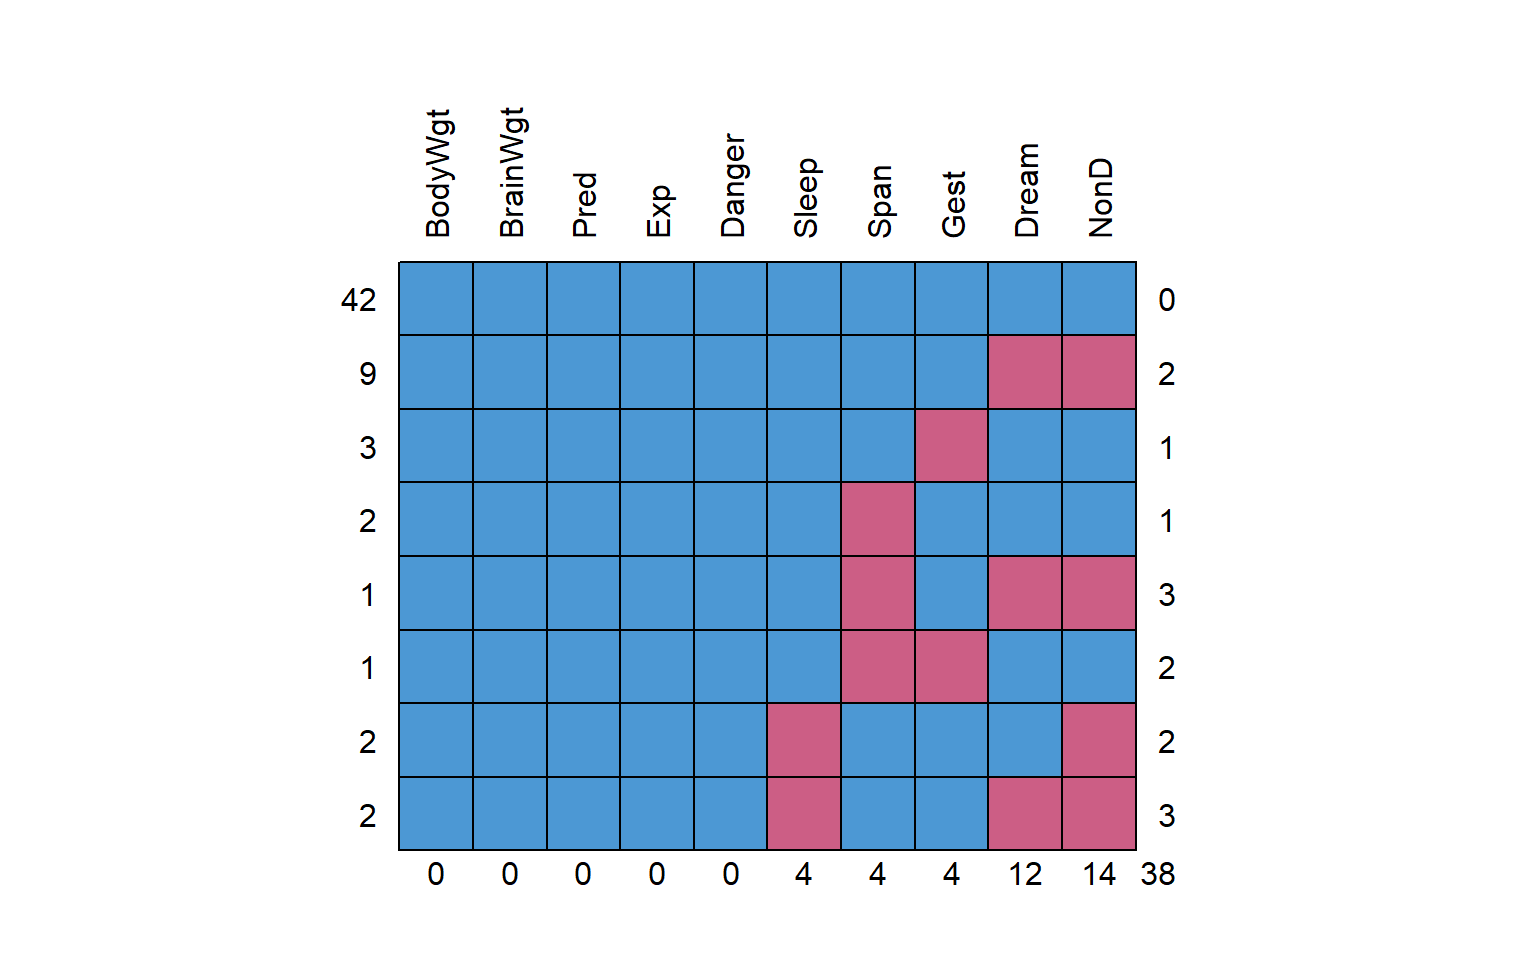
\includegraphics[width=0.8\linewidth]{index_files/figure-latex/unnamed-chunk-7-1}

\begin{verbatim}
##    BodyWgt BrainWgt Pred Exp Danger Sleep Span Gest Dream NonD   
## 42       1        1    1   1      1     1    1    1     1    1  0
## 9        1        1    1   1      1     1    1    1     0    0  2
## 3        1        1    1   1      1     1    1    0     1    1  1
## 2        1        1    1   1      1     1    0    1     1    1  1
## 1        1        1    1   1      1     1    0    1     0    0  3
## 1        1        1    1   1      1     1    0    0     1    1  2
## 2        1        1    1   1      1     0    1    1     1    0  2
## 2        1        1    1   1      1     0    1    1     0    0  3
##          0        0    0   0      0     4    4    4    12   14 38
\end{verbatim}

\begin{Shaded}
\begin{Highlighting}[]
\NormalTok{mice}\SpecialCharTok{::}\FunctionTok{md.pairs}\NormalTok{(sleep)}
\end{Highlighting}
\end{Shaded}

\begin{verbatim}
## $rr
##          BodyWgt BrainWgt NonD Dream Sleep Span Gest Pred Exp Danger
## BodyWgt       62       62   48    50    58   58   58   62  62     62
## BrainWgt      62       62   48    50    58   58   58   62  62     62
## NonD          48       48   48    48    48   45   44   48  48     48
## Dream         50       50   48    50    48   47   46   50  50     50
## Sleep         58       58   48    48    58   54   54   58  58     58
## Span          58       58   45    47    54   58   55   58  58     58
## Gest          58       58   44    46    54   55   58   58  58     58
## Pred          62       62   48    50    58   58   58   62  62     62
## Exp           62       62   48    50    58   58   58   62  62     62
## Danger        62       62   48    50    58   58   58   62  62     62
## 
## $rm
##          BodyWgt BrainWgt NonD Dream Sleep Span Gest Pred Exp Danger
## BodyWgt        0        0   14    12     4    4    4    0   0      0
## BrainWgt       0        0   14    12     4    4    4    0   0      0
## NonD           0        0    0     0     0    3    4    0   0      0
## Dream          0        0    2     0     2    3    4    0   0      0
## Sleep          0        0   10    10     0    4    4    0   0      0
## Span           0        0   13    11     4    0    3    0   0      0
## Gest           0        0   14    12     4    3    0    0   0      0
## Pred           0        0   14    12     4    4    4    0   0      0
## Exp            0        0   14    12     4    4    4    0   0      0
## Danger         0        0   14    12     4    4    4    0   0      0
## 
## $mr
##          BodyWgt BrainWgt NonD Dream Sleep Span Gest Pred Exp Danger
## BodyWgt        0        0    0     0     0    0    0    0   0      0
## BrainWgt       0        0    0     0     0    0    0    0   0      0
## NonD          14       14    0     2    10   13   14   14  14     14
## Dream         12       12    0     0    10   11   12   12  12     12
## Sleep          4        4    0     2     0    4    4    4   4      4
## Span           4        4    3     3     4    0    3    4   4      4
## Gest           4        4    4     4     4    3    0    4   4      4
## Pred           0        0    0     0     0    0    0    0   0      0
## Exp            0        0    0     0     0    0    0    0   0      0
## Danger         0        0    0     0     0    0    0    0   0      0
## 
## $mm
##          BodyWgt BrainWgt NonD Dream Sleep Span Gest Pred Exp Danger
## BodyWgt        0        0    0     0     0    0    0    0   0      0
## BrainWgt       0        0    0     0     0    0    0    0   0      0
## NonD           0        0   14    12     4    1    0    0   0      0
## Dream          0        0   12    12     2    1    0    0   0      0
## Sleep          0        0    4     2     4    0    0    0   0      0
## Span           0        0    1     1     0    4    1    0   0      0
## Gest           0        0    0     0     0    1    4    0   0      0
## Pred           0        0    0     0     0    0    0    0   0      0
## Exp            0        0    0     0     0    0    0    0   0      0
## Danger         0        0    0     0     0    0    0    0   0      0
\end{verbatim}

En estos gráficos y tablas observamos las diferentes combinaciones de
valores perdidos que tenemos para nuestras variables. Ahora, podemos
responder las siguiente preguntas:

\begin{itemize}
\tightlist
\item
  ¿Cuantas observaciones no tienen nigún valor perdido?
\item
  ¿Cuantas observaciones no tienen nigún valor perdido?
\end{itemize}

Visualización de datos perdidos

\begin{Shaded}
\begin{Highlighting}[]
\NormalTok{sleep\_aggr }\OtherTok{\textless{}{-}}\NormalTok{ VIM}\SpecialCharTok{::}\FunctionTok{aggr}\NormalTok{(sleep, }\AttributeTok{col =}\NormalTok{ mice}\SpecialCharTok{::}\FunctionTok{mdc}\NormalTok{(}\DecValTok{1}\SpecialCharTok{:}\DecValTok{2}\NormalTok{), }\AttributeTok{numbers =} \ConstantTok{TRUE}\NormalTok{, }
                        \AttributeTok{sortVars =} \ConstantTok{TRUE}\NormalTok{, }\AttributeTok{labels =} \FunctionTok{names}\NormalTok{(sleep),}
                        \AttributeTok{cex.axis=} \FloatTok{0.7}\NormalTok{, }\AttributeTok{gap =} \DecValTok{3}\NormalTok{,}
                        \AttributeTok{ylab =} \FunctionTok{c}\NormalTok{(}\StringTok{"Proporción de Pérdida"}\NormalTok{,}
                                 \StringTok{"Patrón de Pérdida"}\NormalTok{))}
\end{Highlighting}
\end{Shaded}

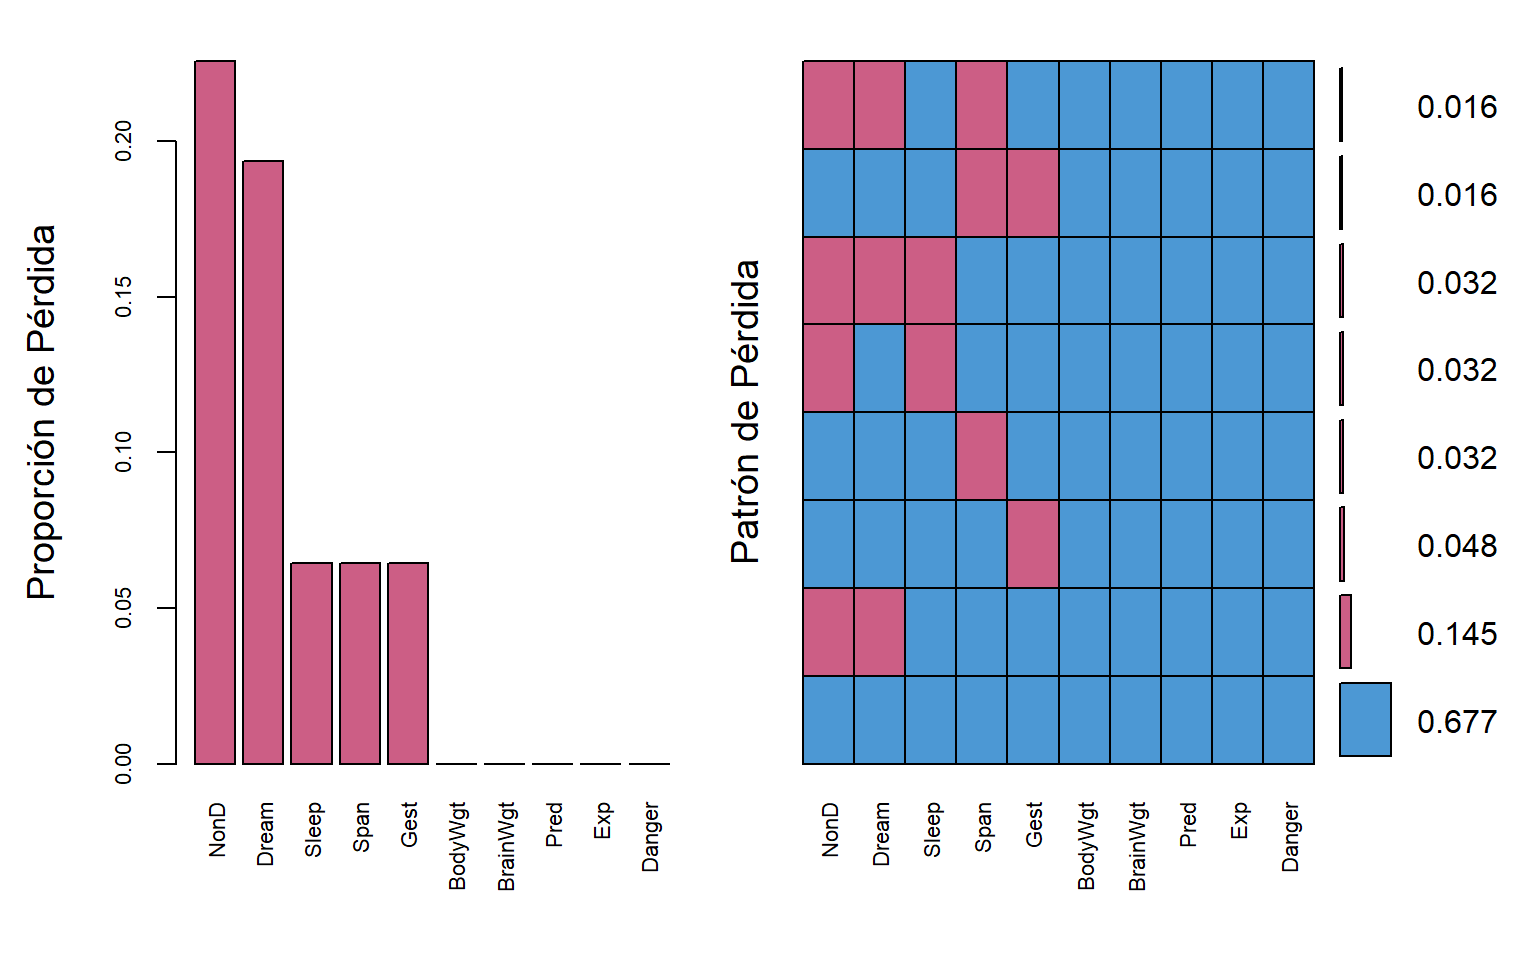
\includegraphics{index_files/figure-latex/unnamed-chunk-8-1.pdf}

\begin{verbatim}
## 
##  Variables sorted by number of missings: 
##  Variable      Count
##      NonD 0.22580645
##     Dream 0.19354839
##     Sleep 0.06451613
##      Span 0.06451613
##      Gest 0.06451613
##   BodyWgt 0.00000000
##  BrainWgt 0.00000000
##      Pred 0.00000000
##       Exp 0.00000000
##    Danger 0.00000000
\end{verbatim}

Distribución de observaciones completas e incompletas por pares de
variables

\begin{Shaded}
\begin{Highlighting}[]
\NormalTok{VIM}\SpecialCharTok{::}\FunctionTok{marginplot}\NormalTok{(sleep[ , }\FunctionTok{c}\NormalTok{(}\DecValTok{3}\NormalTok{, }\DecValTok{7}\NormalTok{)], }\AttributeTok{pch =} \DecValTok{19}\NormalTok{)}
\end{Highlighting}
\end{Shaded}

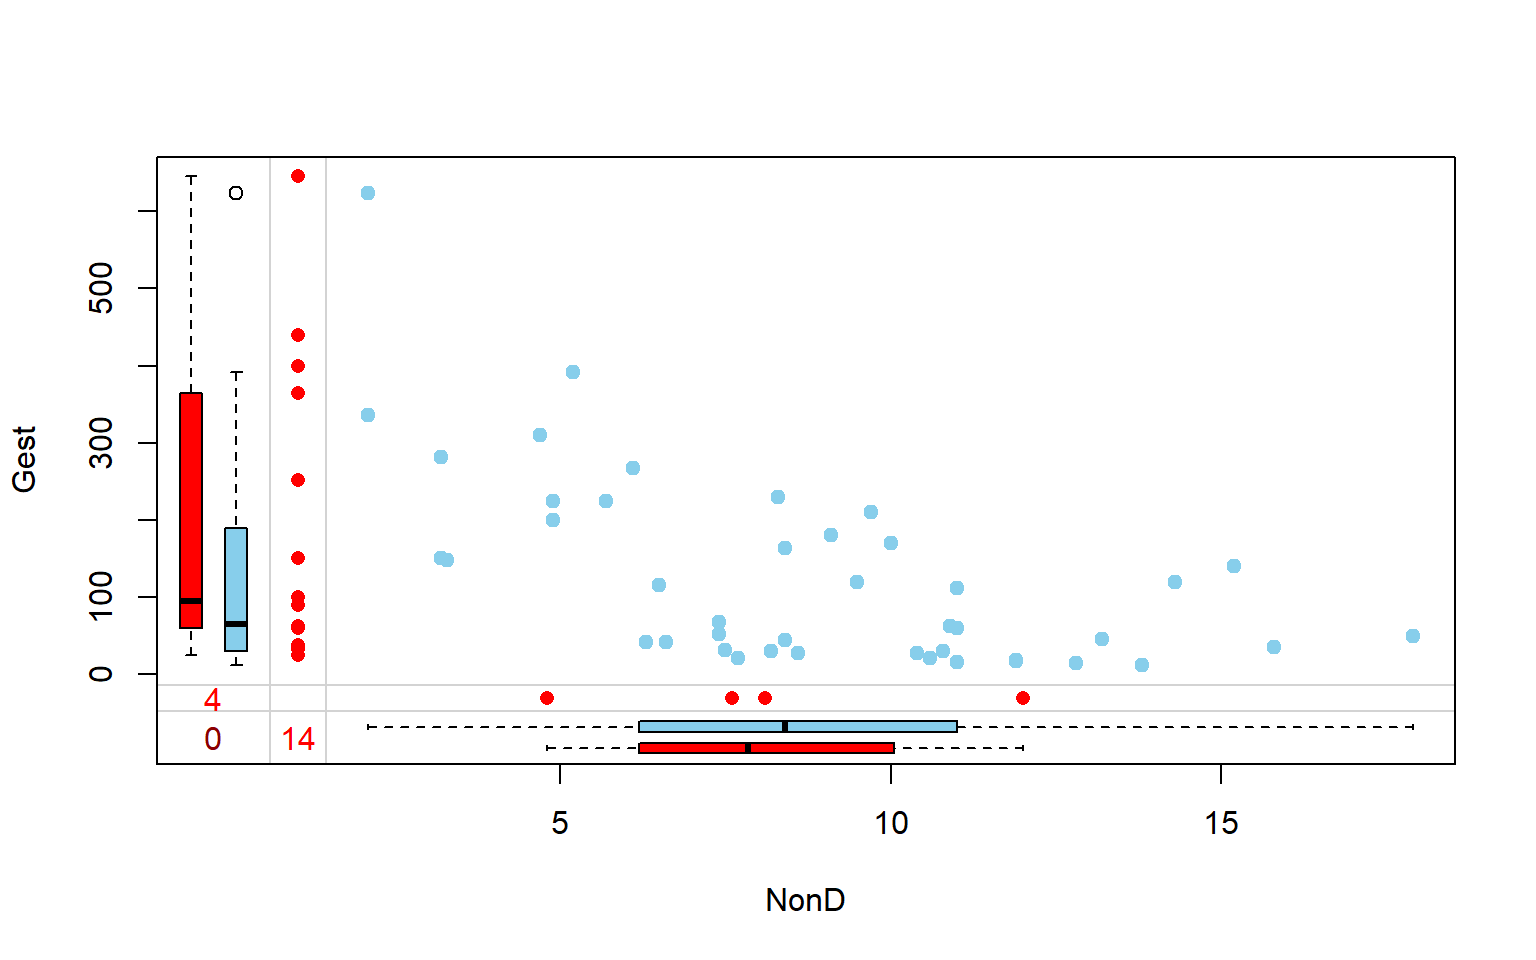
\includegraphics{index_files/figure-latex/unnamed-chunk-9-1.pdf}

\begin{Shaded}
\begin{Highlighting}[]
\NormalTok{VIM}\SpecialCharTok{::}\FunctionTok{marginplot}\NormalTok{(sleep[ , }\FunctionTok{c}\NormalTok{(}\DecValTok{3}\NormalTok{, }\DecValTok{7}\NormalTok{)], }\AttributeTok{col =} \FunctionTok{c}\NormalTok{(}\StringTok{"blue"}\NormalTok{, }\StringTok{"red"}\NormalTok{, }\StringTok{"orange"}\NormalTok{), }\AttributeTok{pch =} \DecValTok{20}\NormalTok{)}
\end{Highlighting}
\end{Shaded}

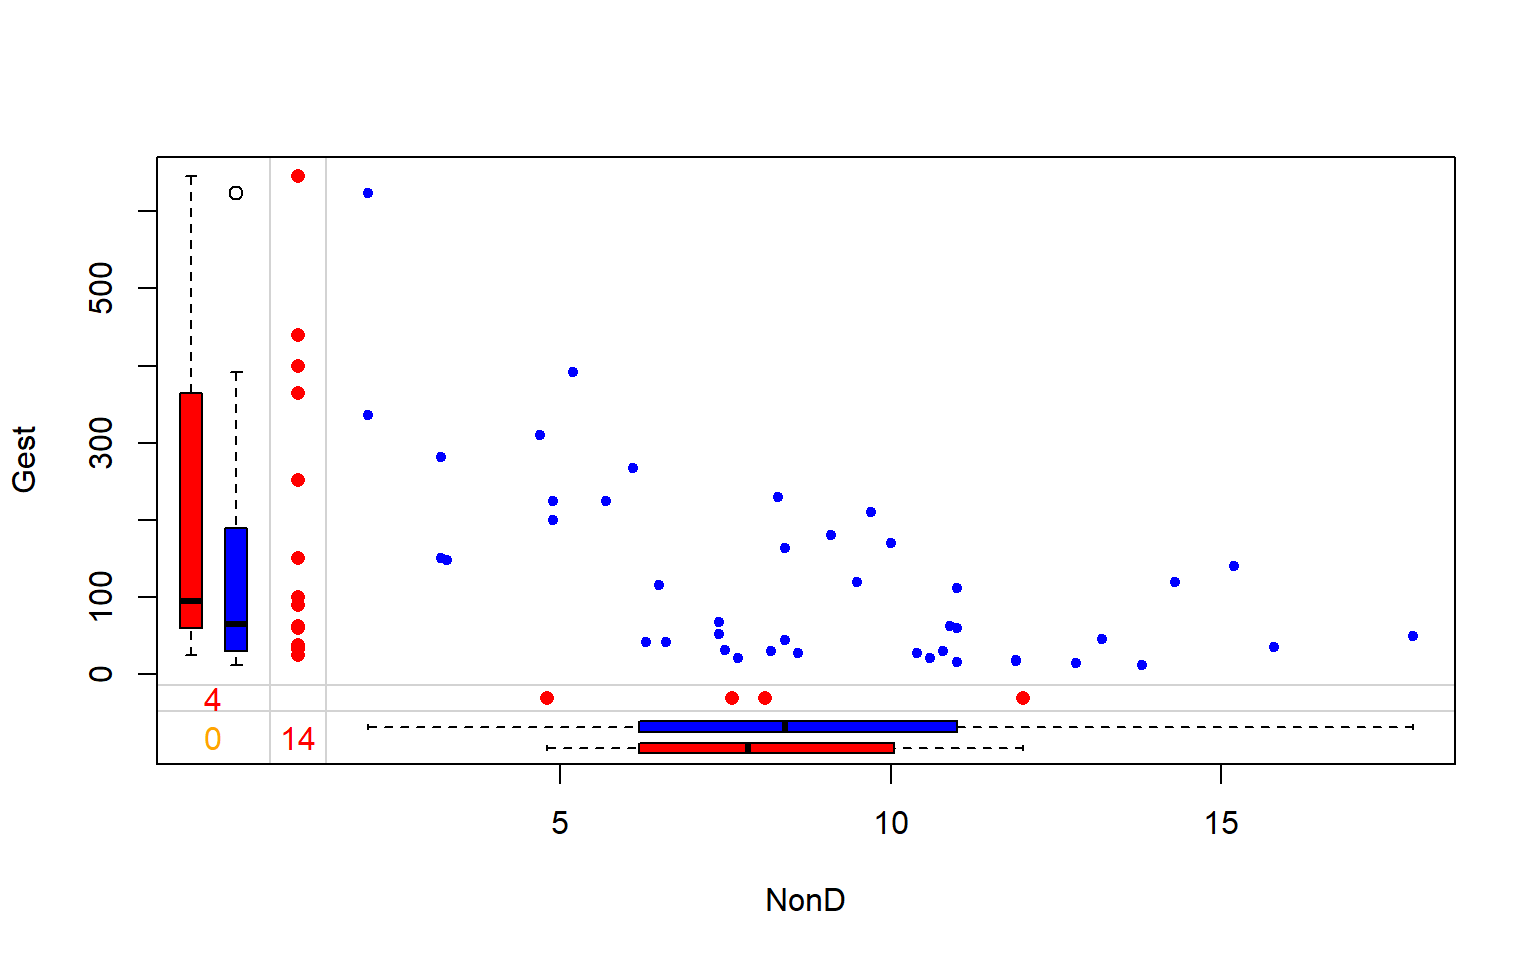
\includegraphics{index_files/figure-latex/unnamed-chunk-9-2.pdf}

Descripción:

\begin{itemize}
\item
  Puntos azules (diagrama de dispersión): individuos con ambos valores
  de las variables.
\item
  Boxplots azules: boxplots de los valores no perdidos de cada variable
\item
  Puntos rojos (Eje X: NonD): individuos con valores perdidos en Gest
  pero observados en NonD.
\item
  Puntos rojos (Eje Y: Gest): individuos con valores perdidos en NonD
  pero observados en Gest.
\item
  Boxplots rojos: Representan la distribución marginal de los puntos
  rojos.
\end{itemize}

Nota: Si los datos perdidos son completamente aleatorios se espera que
los boxplots rojos y azules sean idénticos

\newpage

\hypertarget{imputaciuxf3n-univariada}{%
\section{Imputación Univariada}\label{imputaciuxf3n-univariada}}

\hypertarget{con-la-media.}{%
\subsection{Con la media.}\label{con-la-media.}}

instalamos la librería \texttt{Hmisc} para realizar imputaciones
básicas. La instalación, la realizaremos utilizando el siguiente comando
en la consola: \texttt{install.packages("Hmisc")}.

Luego de completada la instalación, comprobamos cargando el paquete.

\begin{Shaded}
\begin{Highlighting}[]
\FunctionTok{library}\NormalTok{(Hmisc)}
\end{Highlighting}
\end{Shaded}

Si no tenemos mayor información, utilizaremos la media como valor de
imputación. Es una imputación rápida, simple y sencilla.

\begin{Shaded}
\begin{Highlighting}[]
\NormalTok{notas}\SpecialCharTok{$}\NormalTok{nota\_imp }\OtherTok{\textless{}{-}} \FunctionTok{with}\NormalTok{(notas, }\FunctionTok{impute}\NormalTok{(nota, mean))}
\NormalTok{notas}
\end{Highlighting}
\end{Shaded}

\begin{verbatim}
##    nombre nota nota_imp
## 1   Jesus   12 12.00000
## 2   Carla   15 15.00000
## 3 Rodrigo   13 13.00000
## 4  Javier   NA 13.33333
\end{verbatim}

\begin{center}\rule{0.5\linewidth}{0.5pt}\end{center}

\hypertarget{con-valor-aleatorio.}{%
\subsection{Con valor aleatorio.}\label{con-valor-aleatorio.}}

Utilizamos un valor aleatorio como valor de imputación: Se selecciona
aleatoriamente a partir de los valores no perdidos. Simple y útil en
caso de MCAR.

\begin{Shaded}
\begin{Highlighting}[]
\NormalTok{notas}\SpecialCharTok{$}\NormalTok{nota\_imp }\OtherTok{\textless{}{-}} \FunctionTok{with}\NormalTok{(notas, }\FunctionTok{impute}\NormalTok{(nota, }\StringTok{\textquotesingle{}random\textquotesingle{}}\NormalTok{))}
\NormalTok{notas}
\end{Highlighting}
\end{Shaded}

\begin{verbatim}
##    nombre nota nota_imp
## 1   Jesus   12       12
## 2   Carla   15       15
## 3 Rodrigo   13       13
## 4  Javier   NA       15
\end{verbatim}

\begin{center}\rule{0.5\linewidth}{0.5pt}\end{center}

\hypertarget{con-un-valor-especuxedfico.}{%
\subsection{Con un valor
específico.}\label{con-un-valor-especuxedfico.}}

Si tenemos información específica, o resulta conveniente, podemos
imputar los datos perdidos con un valor específico.

\begin{Shaded}
\begin{Highlighting}[]
\NormalTok{notas}\SpecialCharTok{$}\NormalTok{nota\_imp }\OtherTok{\textless{}{-}} \FunctionTok{with}\NormalTok{(notas, }\FunctionTok{impute}\NormalTok{(nota, }\DecValTok{99}\NormalTok{))}
\NormalTok{notas}
\end{Highlighting}
\end{Shaded}

\begin{verbatim}
##    nombre nota nota_imp
## 1   Jesus   12       12
## 2   Carla   15       15
## 3 Rodrigo   13       13
## 4  Javier   NA       99
\end{verbatim}

\begin{center}\rule{0.5\linewidth}{0.5pt}\end{center}

\hypertarget{manualmente}{%
\subsection{Manualmente}\label{manualmente}}

Por ultimo, la imputación puede realizarse sin el paquete Hmisc de la
siguiente manera:

\begin{Shaded}
\begin{Highlighting}[]
\NormalTok{notas}\SpecialCharTok{$}\NormalTok{nota[}\FunctionTok{is.na}\NormalTok{(notas}\SpecialCharTok{$}\NormalTok{nota)] }\OtherTok{\textless{}{-}} \FunctionTok{mean}\NormalTok{(notas}\SpecialCharTok{$}\NormalTok{nota, }\AttributeTok{na.rm =}\NormalTok{ T)}
\NormalTok{notas}
\end{Highlighting}
\end{Shaded}

\begin{verbatim}
##    nombre     nota nota_imp
## 1   Jesus 12.00000       12
## 2   Carla 15.00000       15
## 3 Rodrigo 13.00000       13
## 4  Javier 13.33333       99
\end{verbatim}

\hypertarget{imputaciuxf3n-multivariada}{%
\section{Imputación Multivariada}\label{imputaciuxf3n-multivariada}}

\hypertarget{por-regresiuxf3n-lineal.}{%
\subsection{Por regresión lineal.}\label{por-regresiuxf3n-lineal.}}

Con la librería mice. Esta librería sirve para imputación múltiple pero
podemos usarla también para imputación simple si definimos \emph{m=1}.

\begin{Shaded}
\begin{Highlighting}[]
\FunctionTok{library}\NormalTok{(mice) }
\NormalTok{imp }\OtherTok{\textless{}{-}} \FunctionTok{mice}\NormalTok{(sleep, }\AttributeTok{method =} \StringTok{"norm.predict"}\NormalTok{, }\AttributeTok{m =} \DecValTok{1}\NormalTok{, }\AttributeTok{maxit=}\DecValTok{1}\NormalTok{) }\CommentTok{\# Impute data}
\end{Highlighting}
\end{Shaded}

\begin{verbatim}
## 
##  iter imp variable
##   1   1  NonD  Dream  Sleep  Span  Gest
\end{verbatim}

\begin{Shaded}
\begin{Highlighting}[]
\NormalTok{imp\_reg }\OtherTok{\textless{}{-}} \FunctionTok{complete}\NormalTok{(imp)}
\end{Highlighting}
\end{Shaded}

Para missings en variables categorícas se puede utilizar regresión
logistica con el argumento \texttt{method="logreg"}. Ejemplo:
\texttt{mice(nhanes2,\ meth\ =\ c("sample",\ "norm.predict",\ "logreg",\ "norm.predict"))}

Para ver otros métodos, podemos ver la documentación de la función mice
escribiendo \texttt{?mice::mice} en la consola.

\hypertarget{por-k-vecinos-muxe1s-cercanos.}{%
\subsection{Por K vecinos más
cercanos.}\label{por-k-vecinos-muxe1s-cercanos.}}

Aplicamos vecions más cercanos y guardamos los resultados en sleep\_imp

\begin{Shaded}
\begin{Highlighting}[]
\FunctionTok{library}\NormalTok{(DMwR)}
\NormalTok{sleep\_imp }\OtherTok{\textless{}{-}}\NormalTok{ DMwR}\SpecialCharTok{::}\FunctionTok{knnImputation}\NormalTok{(sleep)}
\CommentTok{\#View(sleep\_imp)}
\FunctionTok{summary}\NormalTok{(sleep\_imp)}
\end{Highlighting}
\end{Shaded}

\begin{verbatim}
##     BodyWgt            BrainWgt            NonD            Dream      
##  Min.   :   0.005   Min.   :   0.14   Min.   : 2.100   Min.   :0.000  
##  1st Qu.:   0.600   1st Qu.:   4.25   1st Qu.: 5.800   1st Qu.:0.925  
##  Median :   3.342   Median :  17.25   Median : 8.350   Median :1.800  
##  Mean   : 198.790   Mean   : 283.13   Mean   : 8.489   Mean   :1.976  
##  3rd Qu.:  48.202   3rd Qu.: 166.00   3rd Qu.:10.757   3rd Qu.:2.567  
##  Max.   :6654.000   Max.   :5712.00   Max.   :17.900   Max.   :6.600  
##      Sleep            Span              Gest             Pred      
##  Min.   : 2.60   Min.   :  2.000   Min.   : 12.00   Min.   :1.000  
##  1st Qu.: 6.95   1st Qu.:  6.125   1st Qu.: 35.75   1st Qu.:2.000  
##  Median :10.30   Median : 13.350   Median : 65.68   Median :3.000  
##  Mean   :10.43   Mean   : 19.133   Mean   :138.65   Mean   :2.871  
##  3rd Qu.:13.20   3rd Qu.: 27.000   3rd Qu.:196.80   3rd Qu.:4.000  
##  Max.   :19.90   Max.   :100.000   Max.   :645.00   Max.   :5.000  
##       Exp            Danger     
##  Min.   :1.000   Min.   :1.000  
##  1st Qu.:1.000   1st Qu.:1.000  
##  Median :2.000   Median :2.000  
##  Mean   :2.419   Mean   :2.613  
##  3rd Qu.:4.000   3rd Qu.:4.000  
##  Max.   :5.000   Max.   :5.000
\end{verbatim}

¿Hay datos perdidos ahora?

\begin{Shaded}
\begin{Highlighting}[]
\FunctionTok{apply}\NormalTok{(sleep\_imp, }\DecValTok{2}\NormalTok{, }\ControlFlowTok{function}\NormalTok{(x)\{}\FunctionTok{sum}\NormalTok{(}\FunctionTok{is.na}\NormalTok{(x))\})}
\end{Highlighting}
\end{Shaded}

\begin{verbatim}
##  BodyWgt BrainWgt     NonD    Dream    Sleep     Span     Gest     Pred 
##        0        0        0        0        0        0        0        0 
##      Exp   Danger 
##        0        0
\end{verbatim}

\hypertarget{por-bosques-aleatorios.}{%
\subsection{Por bosques aleatorios.}\label{por-bosques-aleatorios.}}

\begin{Shaded}
\begin{Highlighting}[]
\FunctionTok{library}\NormalTok{(missForest)}
\NormalTok{sleep\_imp\_rf }\OtherTok{\textless{}{-}} \FunctionTok{missForest}\NormalTok{(sleep)}
\end{Highlighting}
\end{Shaded}

\begin{verbatim}
##   missForest iteration 1 in progress...done!
##   missForest iteration 2 in progress...done!
##   missForest iteration 3 in progress...done!
\end{verbatim}

\begin{Shaded}
\begin{Highlighting}[]
\FunctionTok{print}\NormalTok{(sleep\_imp}\SpecialCharTok{$}\NormalTok{NonD, }\AttributeTok{digits =} \DecValTok{3}\NormalTok{)}
\end{Highlighting}
\end{Shaded}

\begin{verbatim}
##  [1]  2.28  6.30 10.28 10.63  2.10  9.10 15.80  5.20 10.90  8.30 11.00  3.20
## [13]  7.60  4.20  6.30  8.60  6.60  9.50  4.80 12.00  4.97  3.30 11.00  8.17
## [25]  4.70 10.54 10.40  7.40  2.10  9.21  7.65  7.70 17.90  6.10  8.20  8.40
## [37] 11.90 10.80 13.80 14.30  5.25 15.20 10.00 11.90  6.50  7.50 10.50 10.60
## [49]  7.40  8.40  5.70  4.90  4.60  3.20  9.66  8.10 11.00  4.90 13.20  9.70
## [61] 12.80 12.04
\end{verbatim}

\hypertarget{mice}{%
\subsection{MICE}\label{mice}}

\begin{quote}
MICE: \emph{Multivariate Imputation by Chained Equations}
\end{quote}

Utilizaremos la metodología MICE: Multivariate Imputation by Chained
Equations para realizar imputación multivariada.

La imputación con MICE puede ser simple o múltiple. Simple si solo se
imputa el dataset inicial; y múltiple cuando se crean multiples datasets
con diferentes imputaciones.

\begin{Shaded}
\begin{Highlighting}[]
\FunctionTok{library}\NormalTok{(VIM)}
\FunctionTok{library}\NormalTok{(mice)}
\end{Highlighting}
\end{Shaded}

\hypertarget{imputaciuxf3n-muxfaltiple}{%
\section{Imputación Múltiple}\label{imputaciuxf3n-muxfaltiple}}

\hypertarget{mice-1}{%
\subsection{MICE}\label{mice-1}}

Utilizamos el paquete MICE: Imputación Multivariada por Chained
Equations para realizar la imputación múltiple.

\begin{Shaded}
\begin{Highlighting}[]
\FunctionTok{library}\NormalTok{(mice)}
\end{Highlighting}
\end{Shaded}

La imputación se realiza con estas líneas de código:

\begin{Shaded}
\begin{Highlighting}[]
\NormalTok{imp1 }\OtherTok{\textless{}{-}} \FunctionTok{mice}\NormalTok{(sleep, }\AttributeTok{m =} \DecValTok{5}\NormalTok{, }\AttributeTok{seed =} \DecValTok{2}\NormalTok{)}
\end{Highlighting}
\end{Shaded}

\begin{verbatim}
## 
##  iter imp variable
##   1   1  NonD  Dream  Sleep  Span  Gest
##   1   2  NonD  Dream  Sleep  Span  Gest
##   1   3  NonD  Dream  Sleep  Span  Gest
##   1   4  NonD  Dream  Sleep  Span  Gest
##   1   5  NonD  Dream  Sleep  Span  Gest
##   2   1  NonD  Dream  Sleep  Span  Gest
##   2   2  NonD  Dream  Sleep  Span  Gest
##   2   3  NonD  Dream  Sleep  Span  Gest
##   2   4  NonD  Dream  Sleep  Span  Gest
##   2   5  NonD  Dream  Sleep  Span  Gest
##   3   1  NonD  Dream  Sleep  Span  Gest
##   3   2  NonD  Dream  Sleep  Span  Gest
##   3   3  NonD  Dream  Sleep  Span  Gest
##   3   4  NonD  Dream  Sleep  Span  Gest
##   3   5  NonD  Dream  Sleep  Span  Gest
##   4   1  NonD  Dream  Sleep  Span  Gest
##   4   2  NonD  Dream  Sleep  Span  Gest
##   4   3  NonD  Dream  Sleep  Span  Gest
##   4   4  NonD  Dream  Sleep  Span  Gest
##   4   5  NonD  Dream  Sleep  Span  Gest
##   5   1  NonD  Dream  Sleep  Span  Gest
##   5   2  NonD  Dream  Sleep  Span  Gest
##   5   3  NonD  Dream  Sleep  Span  Gest
##   5   4  NonD  Dream  Sleep  Span  Gest
##   5   5  NonD  Dream  Sleep  Span  Gest
\end{verbatim}

\begin{Shaded}
\begin{Highlighting}[]
\NormalTok{imp1}
\end{Highlighting}
\end{Shaded}

\begin{verbatim}
## Class: mids
## Number of multiple imputations:  5 
## Imputation methods:
##  BodyWgt BrainWgt     NonD    Dream    Sleep     Span     Gest     Pred 
##       ""       ""    "pmm"    "pmm"    "pmm"    "pmm"    "pmm"       "" 
##      Exp   Danger 
##       ""       "" 
## PredictorMatrix:
##          BodyWgt BrainWgt NonD Dream Sleep Span Gest Pred Exp Danger
## BodyWgt        0        1    1     1     1    1    1    1   1      1
## BrainWgt       1        0    1     1     1    1    1    1   1      1
## NonD           1        1    0     1     1    1    1    1   1      1
## Dream          1        1    1     0     1    1    1    1   1      1
## Sleep          1        1    1     1     0    1    1    1   1      1
## Span           1        1    1     1     1    0    1    1   1      1
## Number of logged events:  11 
##   it im  dep meth   out
## 1  1  5 Span  pmm Sleep
## 2  1  5 Gest  pmm Sleep
## 3  3  2 Span  pmm Sleep
## 4  3  5 Span  pmm Sleep
## 5  3  5 Gest  pmm Sleep
## 6  4  1 Span  pmm Sleep
\end{verbatim}

El argumento m=5 indica que se crearan 5 datasets de imputaciones.

Verificamos el métodos de imputación utilizado:

\begin{Shaded}
\begin{Highlighting}[]
\NormalTok{imp1}\SpecialCharTok{$}\NormalTok{method}
\end{Highlighting}
\end{Shaded}

\begin{verbatim}
##  BodyWgt BrainWgt     NonD    Dream    Sleep     Span     Gest     Pred 
##       ""       ""    "pmm"    "pmm"    "pmm"    "pmm"    "pmm"       "" 
##      Exp   Danger 
##       ""       ""
\end{verbatim}

Como vemos, se usó el método pmm (Predictive mean matching): Un método
de imputación semi-parámetrico usado por defecto para variables
continuas. - Selecciona un grupo de candidatos vecino similares y
cercanos, y toma uno aleatoriamente como donador.

Imputaciones para una variable en particular. Veamos el objeto
\textbf{imp1}, que tiene una lista de imputados \textbf{imp} con un set
de imputados para la columna NonD

\begin{Shaded}
\begin{Highlighting}[]
\FunctionTok{head}\NormalTok{(imp1}\SpecialCharTok{$}\NormalTok{imp}\SpecialCharTok{$}\NormalTok{NonD)}
\end{Highlighting}
\end{Shaded}

\begin{verbatim}
##       1    2    3    4    5
## 1   3.2  3.3  2.1  2.1  3.2
## 3  10.0 12.0 10.8 11.9 11.0
## 4  11.0 10.4 12.8 17.9 13.2
## 14  2.1  3.2  3.2  2.1  3.2
## 21 12.8 11.9  7.6  4.7  8.2
## 24  8.4 11.0 11.0 11.0 10.0
\end{verbatim}

Notemos que cada columna representa a un set de valores imputados para
una variable.

\hypertarget{visualizaciuxf3n.}{%
\subsection{Visualización.}\label{visualizaciuxf3n.}}

Estos gráficos nos servirán para revisar si las imputaciones realizadas
son muy variables entre diferentes datasets.

\begin{itemize}
\item
  El primer gráfico muestra los valores perdidos para la variable en el
  eje Y: \textbf{Gest}.
\item
  Se muestran 6 cuadros correspondientes a

  \begin{itemize}
  \tightlist
  \item
    La data original y
  \item
    Los 5 dataset construidos con la imputación multiple.
  \end{itemize}
\item
  En \textbf{rojo} están las observaciones imputadas para la variable
  Gest (variable del eje Y); y en \textbf{azul}, todas las demás
  observaciones.
\item
  Los puntos azules son los datos observados y además imputaciones
  realizadas en la variable \textbf{NonD} (variable del eje X).
\end{itemize}

\begin{Shaded}
\begin{Highlighting}[]
\FunctionTok{library}\NormalTok{(lattice)}
\FunctionTok{xyplot}\NormalTok{(imp1, Gest }\SpecialCharTok{\textasciitilde{}}\NormalTok{ NonD }\SpecialCharTok{|}\NormalTok{ .imp, }\AttributeTok{pch =} \DecValTok{20}\NormalTok{, }\AttributeTok{cex =} \FloatTok{1.4}\NormalTok{)}
\end{Highlighting}
\end{Shaded}

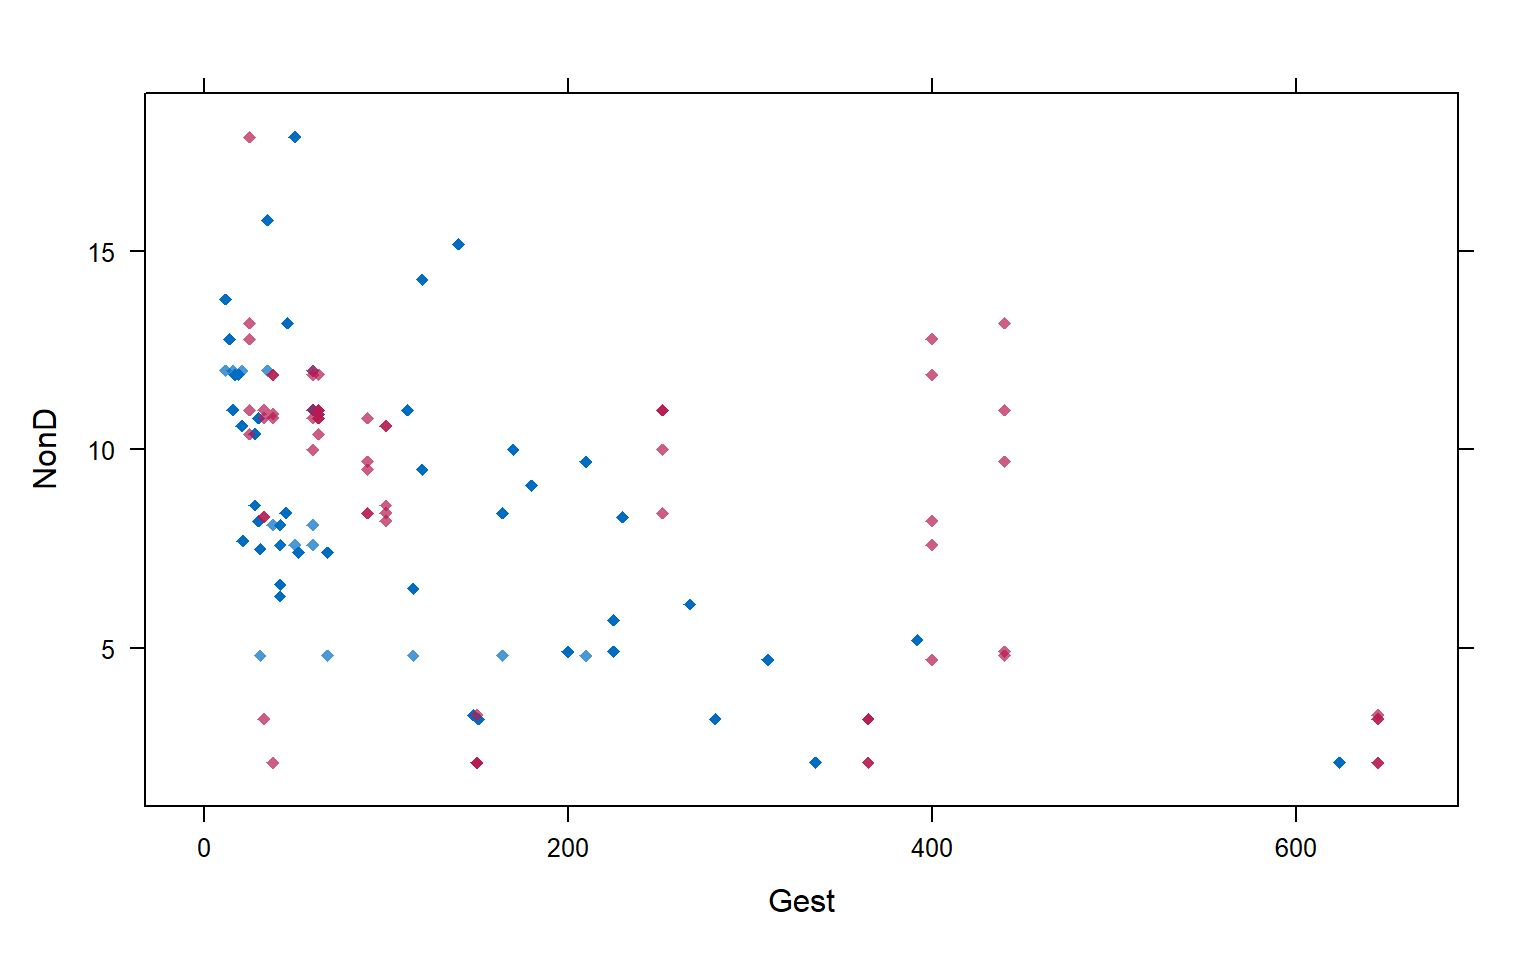
\includegraphics{index_files/figure-latex/unnamed-chunk-27-1.pdf}

\begin{itemize}
\item
  En el siguiente gráfico observamos el mismo tipo de diagrama. Esta vez
  \textbf{enfocado} en el análisis de otra variable: \textbf{NonD} (Note
  la diferencia en la formula utilizada \emph{NonD \textasciitilde{}
  Gest}).
\item
  A partir de los \textbf{puntos rosados} en los diferentes cuadros, se
  observan las variaciones en las imputaciones para \textbf{NonD} en los
  diferentes datasets contruídos durante la imputación múltiple.
\item
  Notemos a partir de estos gráficos que se están imputando valores
  fuera de la nube de puntos creada entre estas dos variables. Aunque
  podría suceder.
\end{itemize}

\begin{Shaded}
\begin{Highlighting}[]
\FunctionTok{xyplot}\NormalTok{(imp1, NonD }\SpecialCharTok{\textasciitilde{}}\NormalTok{ Gest }\SpecialCharTok{|}\NormalTok{ .imp, }\AttributeTok{pch =} \DecValTok{20}\NormalTok{, }\AttributeTok{cex =} \FloatTok{1.4}\NormalTok{)}
\end{Highlighting}
\end{Shaded}

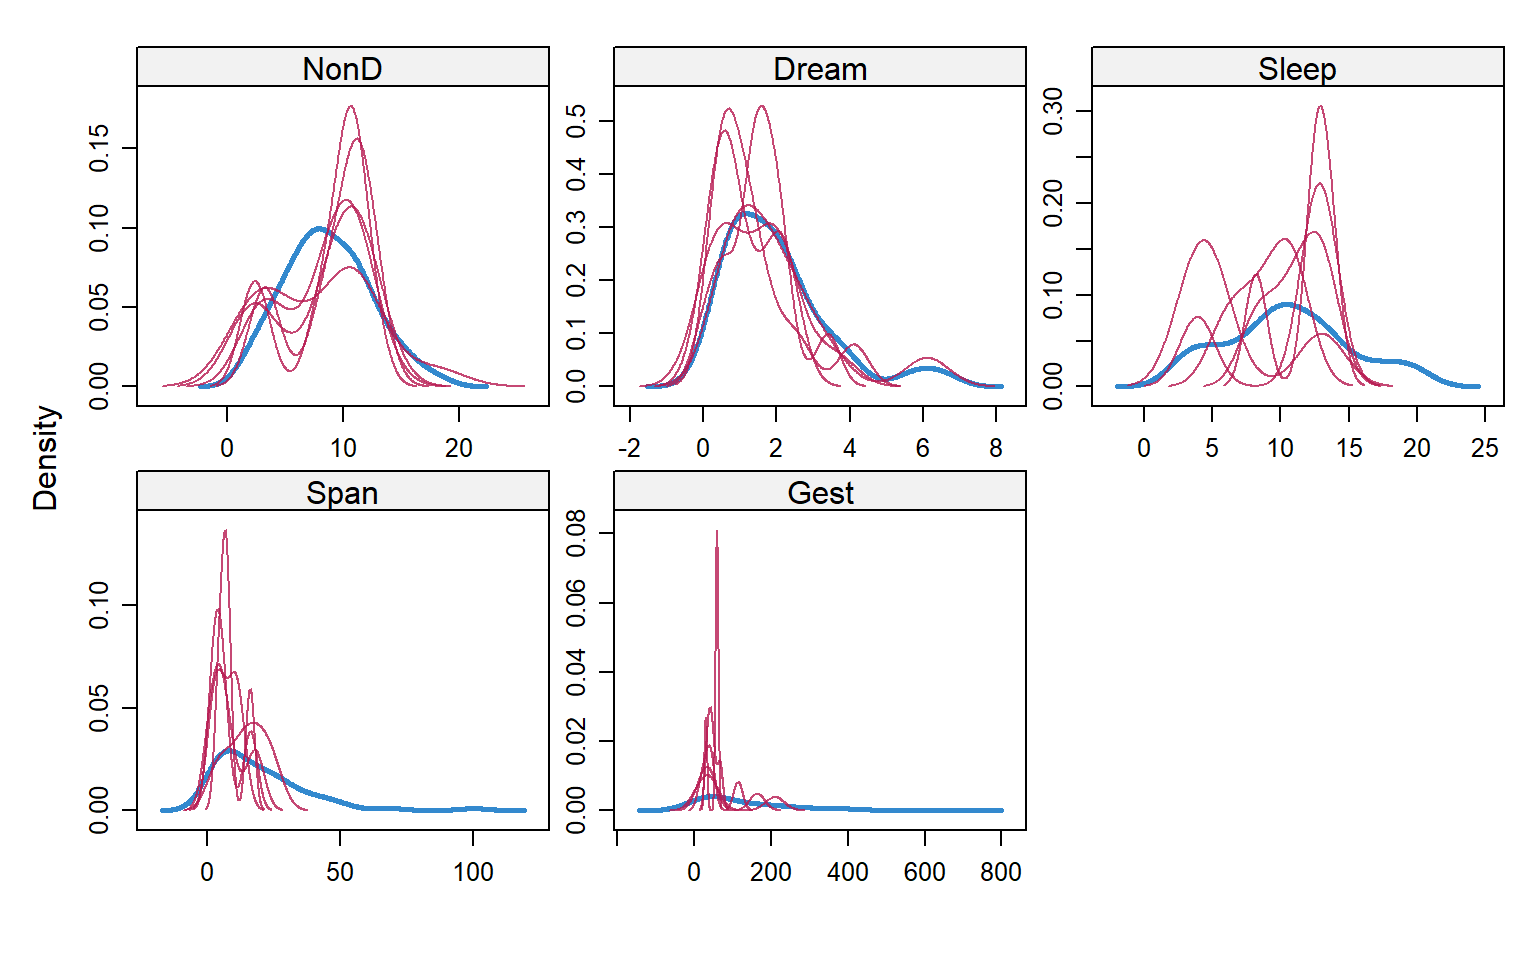
\includegraphics{index_files/figure-latex/unnamed-chunk-28-1.pdf}

Finalmente, para observar los datos de las 5 imputaciones en un solo
gráfico, tenemos el siguiente código.

\textbf{Para la variable Gest}

\begin{Shaded}
\begin{Highlighting}[]
\FunctionTok{xyplot}\NormalTok{(imp1, Gest }\SpecialCharTok{\textasciitilde{}}\NormalTok{ NonD, }\AttributeTok{pch =} \DecValTok{18}\NormalTok{)}
\end{Highlighting}
\end{Shaded}

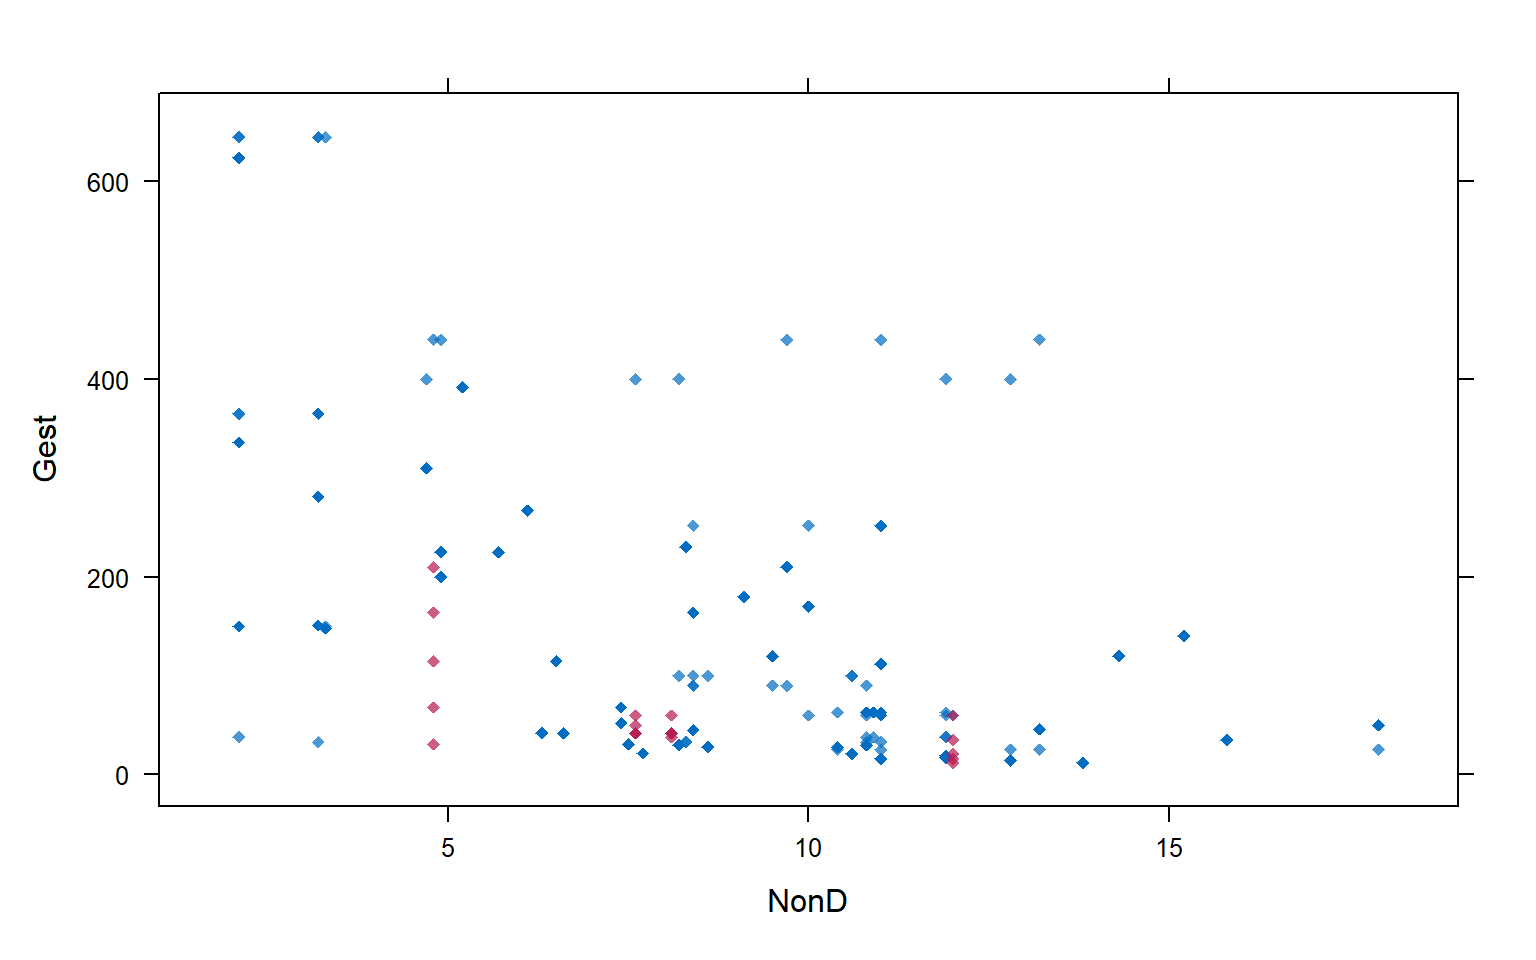
\includegraphics[width=0.7\linewidth]{index_files/figure-latex/unnamed-chunk-29-1}

\textbf{Para la variable NonD}

\begin{Shaded}
\begin{Highlighting}[]
\FunctionTok{xyplot}\NormalTok{(imp1, NonD }\SpecialCharTok{\textasciitilde{}}\NormalTok{ Gest, }\AttributeTok{pch =} \DecValTok{18}\NormalTok{)}
\end{Highlighting}
\end{Shaded}

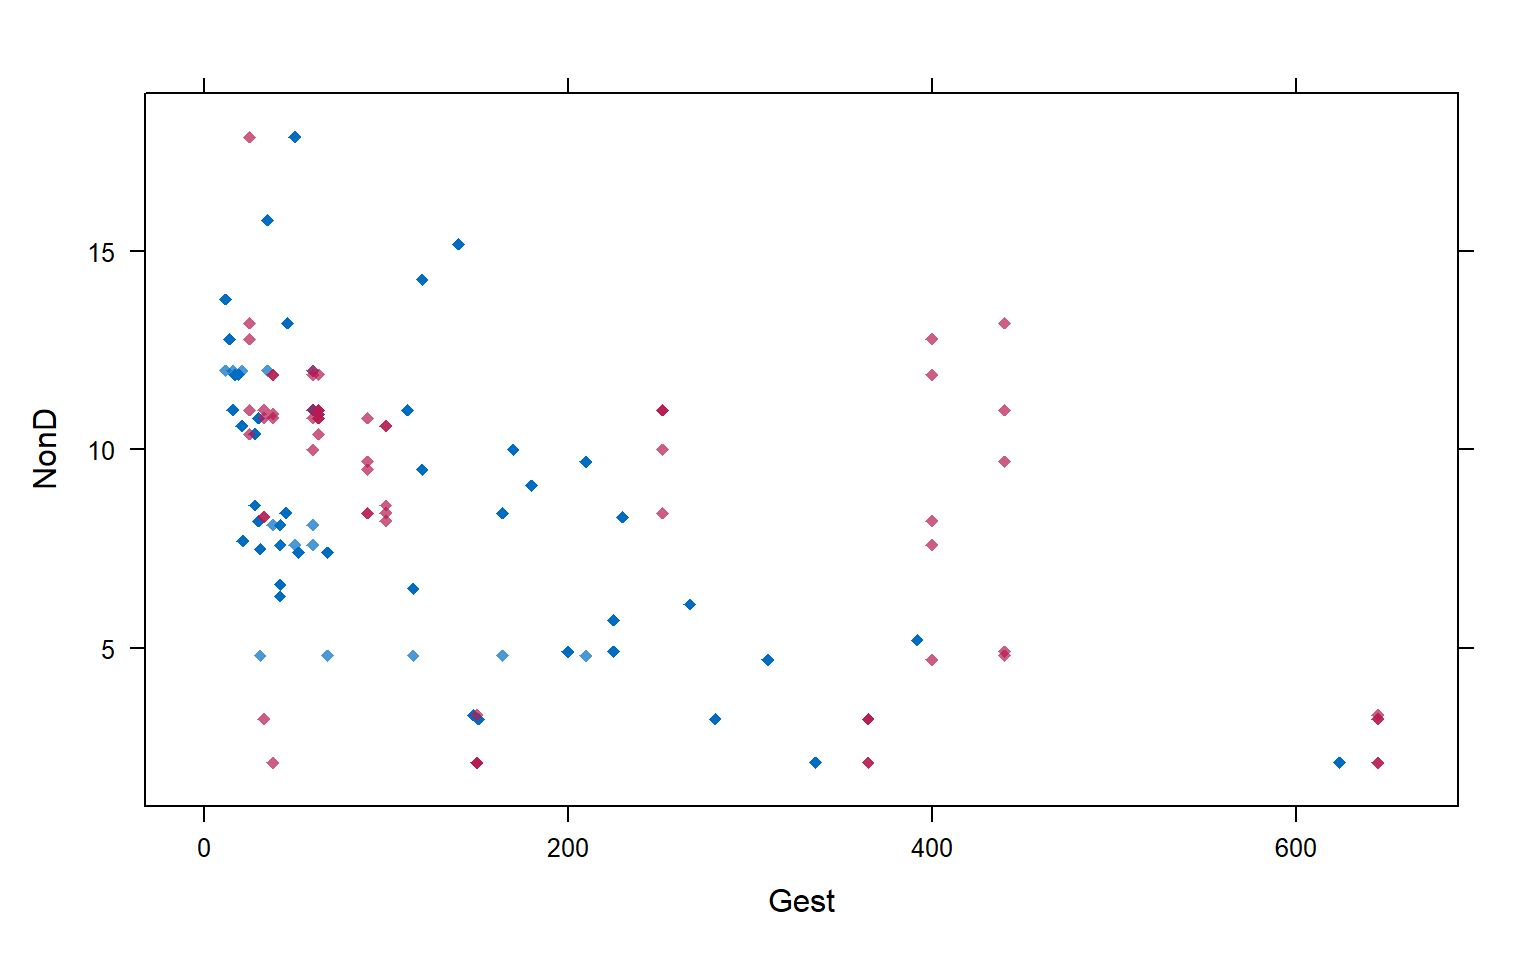
\includegraphics[width=0.7\linewidth]{index_files/figure-latex/unnamed-chunk-30-1}

Ademas, si queremos incluir una tercera variable al análisis podemos
observarla cambiando la formula como el siguiente código.

\begin{Shaded}
\begin{Highlighting}[]
\FunctionTok{xyplot}\NormalTok{(imp1, Gest }\SpecialCharTok{\textasciitilde{}}\NormalTok{ NonD }\SpecialCharTok{+}\NormalTok{ Span , }\AttributeTok{pch =} \DecValTok{18}\NormalTok{)}
\end{Highlighting}
\end{Shaded}

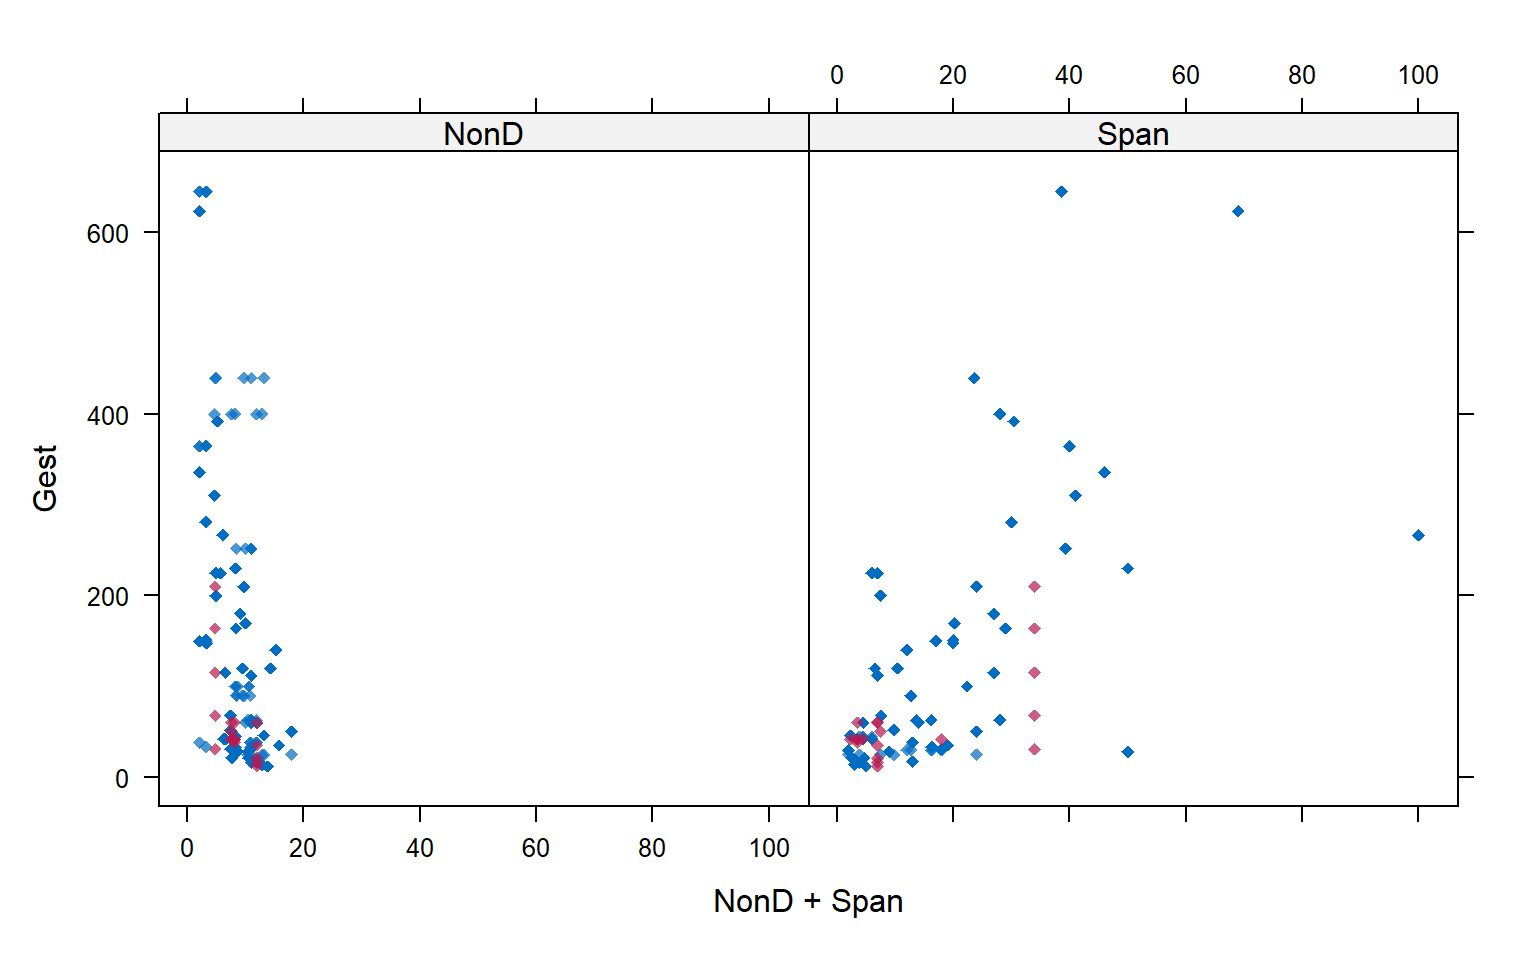
\includegraphics[width=0.9\linewidth]{index_files/figure-latex/unnamed-chunk-31-1}

\begin{itemize}
\item
  Veremos la relación de la variable Gest con Span además de con NonD.
\item
  Los \textbf{puntos rosados} son los valores imputados.
\end{itemize}

Finalmente, utilizaremos un gráfico para la densidad de las
observaciones imputadas en cada dataset.

\begin{itemize}
\item
  Esto nos mostrará si las diferentes imputaciones están concentradas en
  los mismos valores o si cambian entre diferentes datasets.
\item
  Cada densidad está representada en líneas de color rosado y
  representan la densidad para las imputaciones en uno de los 5 datasets
  de la imputación múltiple.
\item
  La densidad en color celeste representa la densidad de los valores
  observados.
\end{itemize}

\begin{Shaded}
\begin{Highlighting}[]
\FunctionTok{densityplot}\NormalTok{(imp1)}
\end{Highlighting}
\end{Shaded}

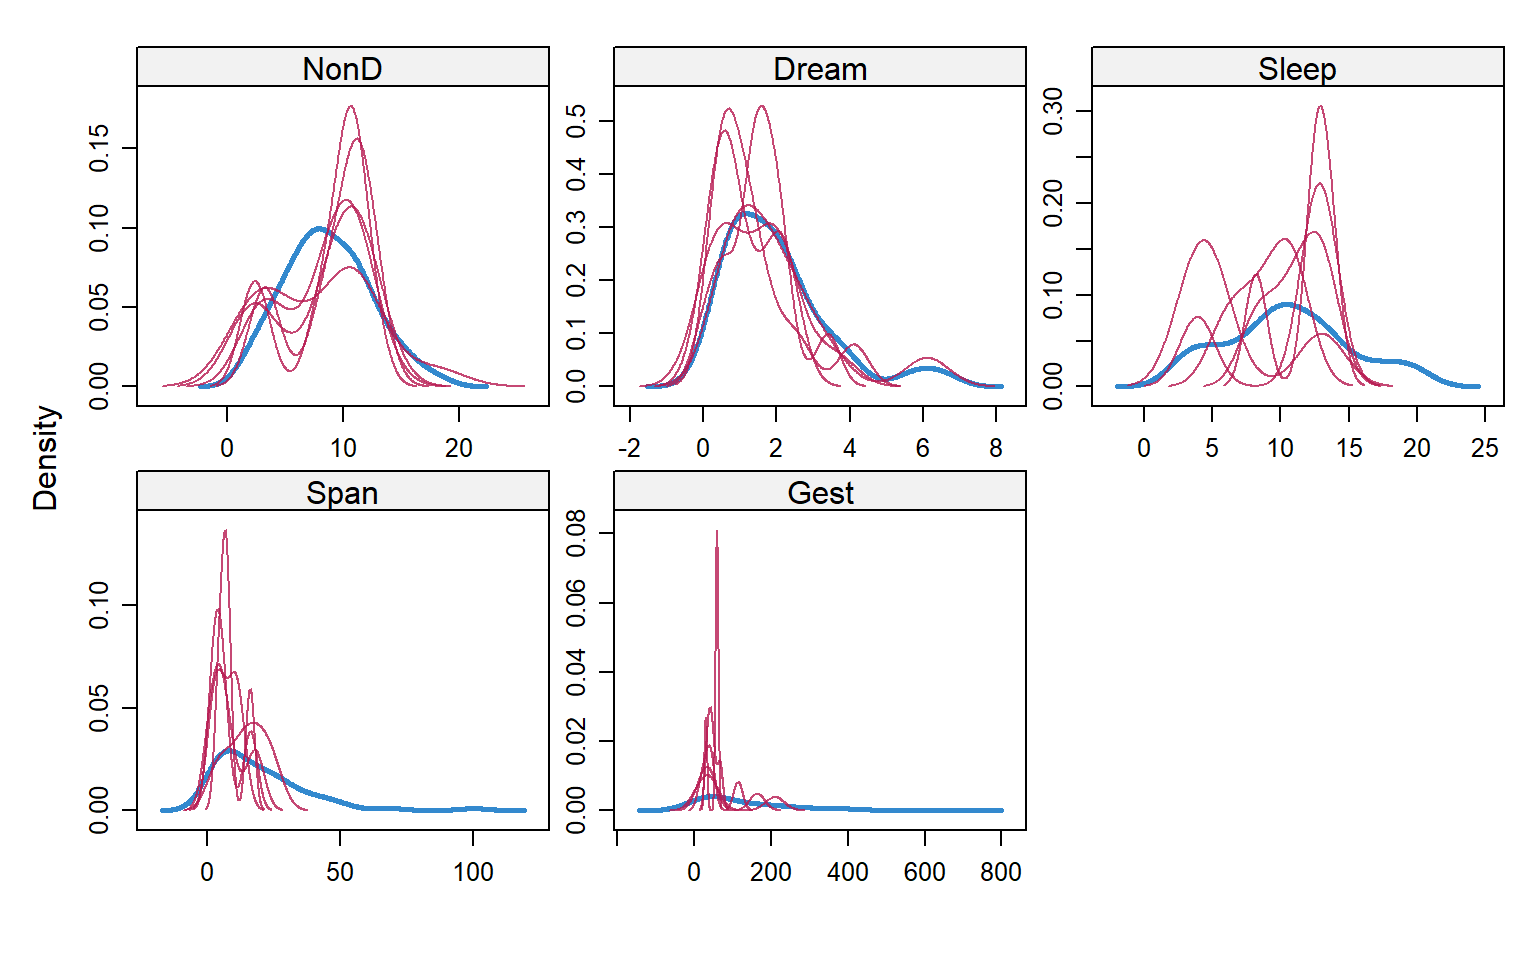
\includegraphics{index_files/figure-latex/unnamed-chunk-32-1.pdf}

\begin{itemize}
\item
  Este gráfico compara la \textbf{densidad de los datos observados
  versus la densidad de los datos imputados}. Se espera que las líneas
  sean similares pero no idénticos.
\item
  Encontrar diferencias entre las diferentes imputaciones indica que las
  \textbf{imputaciones varían} entre diferentes datasets.
\end{itemize}

\textbf{Streeplot}

\begin{itemize}
\item
  El último gráfico llamado \textbf{stripplot} muestra la distribución
  de cada variable y sus valores imputados en los multiples datasets.
\item
  Es \textbf{otra forma} de ver la \textbf{distribución de los
  imputados} en las diferentes muestras.
\end{itemize}

\begin{Shaded}
\begin{Highlighting}[]
\FunctionTok{stripplot}\NormalTok{(imp1, }\AttributeTok{pch =} \DecValTok{20}\NormalTok{)}
\end{Highlighting}
\end{Shaded}

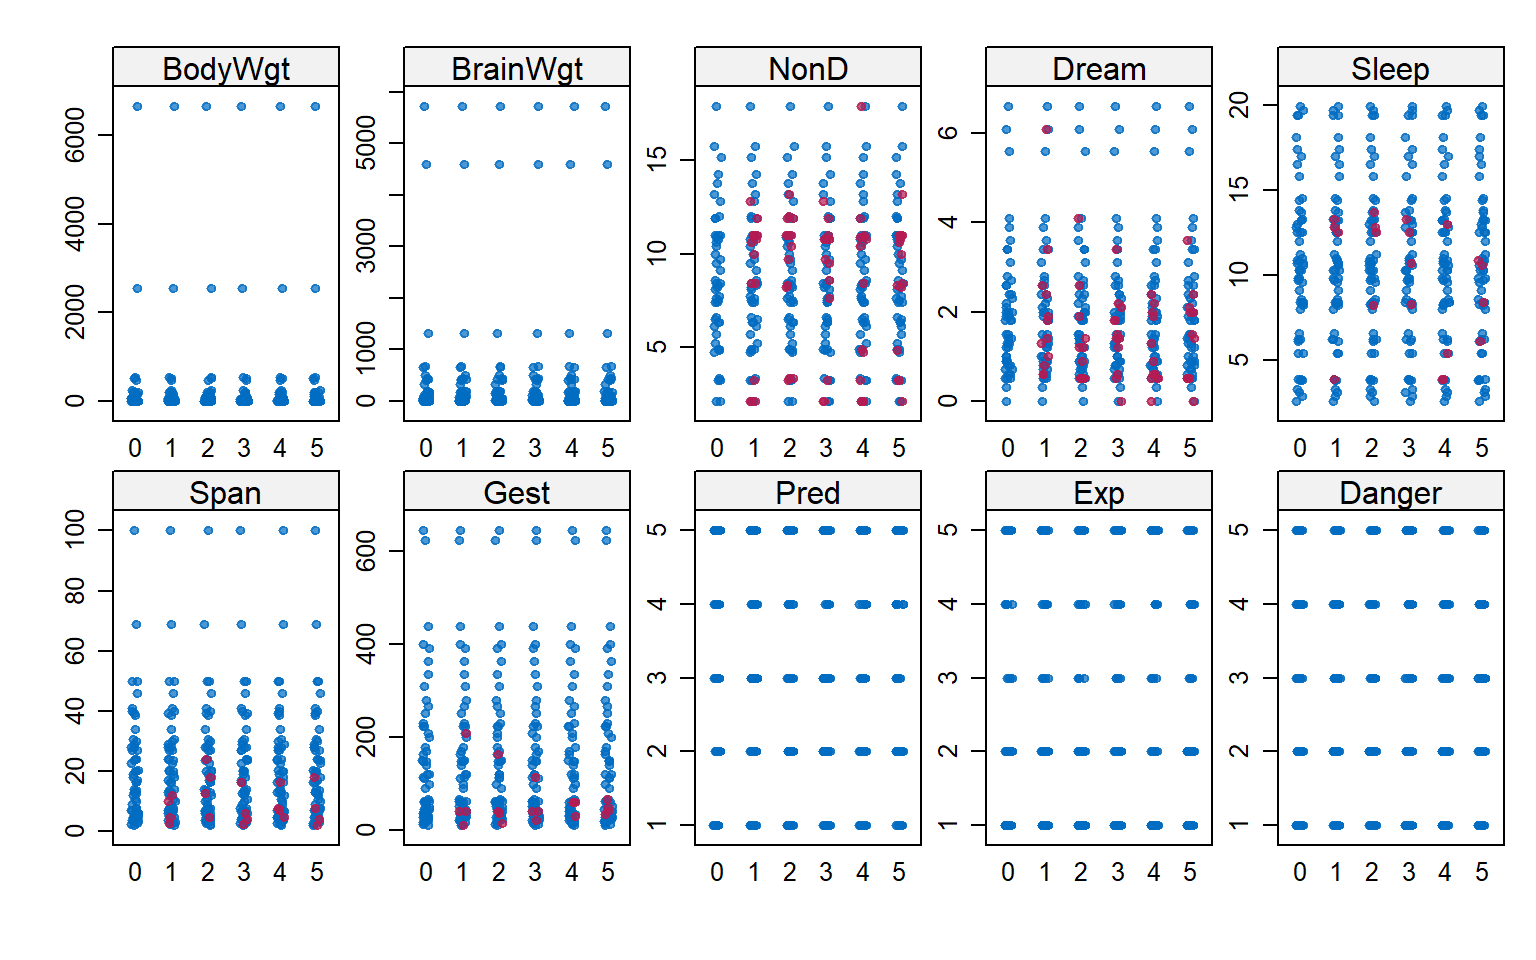
\includegraphics{index_files/figure-latex/unnamed-chunk-33-1.pdf}

\hypertarget{modelamiento}{%
\section{Modelamiento}\label{modelamiento}}

\hypertarget{casos-completos}{%
\subsection{Casos completos}\label{casos-completos}}

El caso más simple y rápido será utilizando solo los datos completos. En
este caso, omitimos las fila con valores perdidos y construimos nuestro
modelo.

\begin{Shaded}
\begin{Highlighting}[]
\NormalTok{ajuste\_cc }\OtherTok{\textless{}{-}} \FunctionTok{lm}\NormalTok{(BodyWgt }\SpecialCharTok{\textasciitilde{}}\NormalTok{ Sleep }\SpecialCharTok{+}\NormalTok{ BrainWgt, }
                \AttributeTok{data =} \FunctionTok{na.omit}\NormalTok{(sleep))}
\FunctionTok{summary}\NormalTok{(ajuste\_cc)}
\end{Highlighting}
\end{Shaded}

\begin{verbatim}
## 
## Call:
## lm(formula = BodyWgt ~ Sleep + BrainWgt, data = na.omit(sleep))
## 
## Residuals:
##     Min      1Q  Median      3Q     Max 
## -616.89   -4.08   11.32   21.49  244.51 
## 
## Coefficients:
##             Estimate Std. Error t value Pr(>|t|)    
## (Intercept)  8.22805   51.15597   0.161    0.873    
## Sleep       -1.98795    4.25534  -0.467    0.643    
## BrainWgt     0.52013    0.02735  19.021   <2e-16 ***
## ---
## Signif. codes:  0 '***' 0.001 '**' 0.01 '*' 0.05 '.' 0.1 ' ' 1
## 
## Residual standard error: 120.8 on 39 degrees of freedom
## Multiple R-squared:  0.9141, Adjusted R-squared:  0.9097 
## F-statistic: 207.6 on 2 and 39 DF,  p-value: < 2.2e-16
\end{verbatim}

\hypertarget{imputaciuxf3n-simple.}{%
\subsection{Imputación simple.}\label{imputaciuxf3n-simple.}}

Despues de una imputación simple, el resultado es un dataset con el
mismo número de filas y columna pero con todos los datos llenos con
algún valor imputado. Al realizar el modelamiento, se utilizan los
resultados de la imputación realizada para entrenar el modelo.

\begin{Shaded}
\begin{Highlighting}[]
\NormalTok{ajuste\_cc }\OtherTok{\textless{}{-}} \FunctionTok{lm}\NormalTok{(BodyWgt }\SpecialCharTok{\textasciitilde{}}\NormalTok{ Sleep }\SpecialCharTok{+}\NormalTok{ BrainWgt, }\AttributeTok{data =}\NormalTok{ imp\_reg)}
\FunctionTok{summary}\NormalTok{(ajuste\_cc)}
\end{Highlighting}
\end{Shaded}

\begin{verbatim}
## 
## Call:
## lm(formula = BodyWgt ~ Sleep + BrainWgt, data = imp_reg)
## 
## Residuals:
##      Min       1Q   Median       3Q      Max 
## -1557.71     4.66    29.05    57.66  1540.90 
## 
## Coefficients:
##               Estimate Std. Error t value Pr(>|t|)    
## (Intercept) -116.74580  107.82251  -1.083    0.283    
## Sleep          5.63502    9.29479   0.606    0.547    
## BrainWgt       0.91233    0.04738  19.254   <2e-16 ***
## ---
## Signif. codes:  0 '***' 0.001 '**' 0.01 '*' 0.05 '.' 0.1 ' ' 1
## 
## Residual standard error: 325.2 on 59 degrees of freedom
## Multiple R-squared:  0.8735, Adjusted R-squared:  0.8692 
## F-statistic: 203.6 on 2 and 59 DF,  p-value: < 2.2e-16
\end{verbatim}

\begin{itemize}
\item
  Nota: Si deseamos utilizar la imputación para nuestra data de
  validación, tenemos que aplicar la metodología y modelos creados para
  la imputación a partir de la data de entrenamiento.
\item
  No deben realizarse modelos para imputaciones con los datos de
  validación sino podríamos sesgar la evaluación del modelo en la data
  de entrenamiento.
\end{itemize}

\hypertarget{imputaciuxf3n-muxfaltiple.}{%
\subsection{Imputación múltiple.}\label{imputaciuxf3n-muxfaltiple.}}

\begin{itemize}
\item
  Luego de una imputación multiple, el entrenamiento del modelo debe
  realizarse en cada uno los múltiples datasets imputados.
\item
  Multiples modelos serán entrenados a partir de los datasets. Es
  nuestra tarea evaluar la \textbf{variabilidad de los modelos} en los
  diferentes conjuntos de datos y analizar el performance conjunto de
  todos ellos. (Cuando los modelos sirven para entender el problema, es
  mejor buscar características estables entre diferentes imputaciones.)
\item
  Ejemplo en R: uso de regresión lineal para los múltiples datasets
  imputados. El resultados del modelo es el siguiente:
\end{itemize}

\begin{Shaded}
\begin{Highlighting}[]
\NormalTok{ajuste\_imp }\OtherTok{\textless{}{-}} \FunctionTok{with}\NormalTok{(imp1, }\FunctionTok{lm}\NormalTok{( BodyWgt }\SpecialCharTok{\textasciitilde{}}\NormalTok{ Sleep }\SpecialCharTok{+}\NormalTok{ BrainWgt))}
\FunctionTok{summary}\NormalTok{(ajuste\_imp)}
\end{Highlighting}
\end{Shaded}

\begin{verbatim}
## # A tibble: 15 x 6
##    term        estimate std.error statistic  p.value  nobs
##    <chr>          <dbl>     <dbl>     <dbl>    <dbl> <int>
##  1 (Intercept) -116.     115.        -1.00  3.20e- 1    62
##  2 Sleep          5.34     9.70       0.550 5.84e- 1    62
##  3 BrainWgt       0.912    0.0476    19.2   5.18e-27    62
##  4 (Intercept) -119.     118.        -1.01  3.16e- 1    62
##  5 Sleep          5.61     9.88       0.568 5.72e- 1    62
##  6 BrainWgt       0.912    0.0478    19.1   6.10e-27    62
##  7 (Intercept) -128.     118.        -1.08  2.86e- 1    62
##  8 Sleep          6.39     9.96       0.642 5.23e- 1    62
##  9 BrainWgt       0.914    0.0480    19.0   7.19e-27    62
## 10 (Intercept) -124.     111.        -1.12  2.69e- 1    62
## 11 Sleep          6.27     9.54       0.657 5.14e- 1    62
## 12 BrainWgt       0.914    0.0478    19.1   5.73e-27    62
## 13 (Intercept) -131.     117.        -1.12  2.68e- 1    62
## 14 Sleep          6.75     9.92       0.680 4.99e- 1    62
## 15 BrainWgt       0.915    0.0480    19.1   6.57e-27    62
\end{verbatim}

Note que es posible utilizar cualquier otra función en lugar de
\texttt{lm()}. El resultado será una lista de modelos para cada dataset.

Performance del modelo en las 5 diferentes imputaciones con la librería
\emph{performance}.

\begin{Shaded}
\begin{Highlighting}[]
\FunctionTok{library}\NormalTok{(performance)}
\FunctionTok{lapply}\NormalTok{(ajuste\_imp}\SpecialCharTok{$}\NormalTok{analyses, performance)}
\end{Highlighting}
\end{Shaded}

\begin{verbatim}
## [[1]]
## # Indices of model performance
## 
## AIC     |     BIC |    R2 | R2 (adj.) |    RMSE |   Sigma
## ---------------------------------------------------------
## 898.227 | 906.736 | 0.873 |     0.869 | 317.447 | 325.418
## 
## [[2]]
## # Indices of model performance
## 
## AIC     |     BIC |    R2 | R2 (adj.) |    RMSE |   Sigma
## ---------------------------------------------------------
## 898.207 | 906.715 | 0.873 |     0.869 | 317.395 | 325.364
## 
## [[3]]
## # Indices of model performance
## 
## AIC     |     BIC |    R2 | R2 (adj.) |    RMSE |   Sigma
## ---------------------------------------------------------
## 898.113 | 906.622 | 0.874 |     0.869 | 317.156 | 325.120
## 
## [[4]]
## # Indices of model performance
## 
## AIC     |     BIC |    R2 | R2 (adj.) |    RMSE |   Sigma
## ---------------------------------------------------------
## 898.092 | 906.601 | 0.874 |     0.869 | 317.103 | 325.065
## 
## [[5]]
## # Indices of model performance
## 
## AIC     |     BIC |    R2 | R2 (adj.) |    RMSE |   Sigma
## ---------------------------------------------------------
## 898.060 | 906.569 | 0.874 |     0.869 | 317.020 | 324.980
\end{verbatim}

Finalmente, el análisis de resultados se realizará combinando los
resultados de cada modelos. En nuestro caso, se juntan los coeficientes
y errores estándares de los 5 modelos de regresión.

\begin{Shaded}
\begin{Highlighting}[]
\NormalTok{ajuste\_comb }\OtherTok{\textless{}{-}} \FunctionTok{pool}\NormalTok{(ajuste\_imp)}
\FunctionTok{summary}\NormalTok{(ajuste\_comb)}
\end{Highlighting}
\end{Shaded}

\begin{verbatim}
##          term     estimate   std.error  statistic       df   p.value
## 1 (Intercept) -123.4775543 116.1456478 -1.0631268 56.89702 0.2922159
## 2       Sleep    6.0728040   9.8226090  0.6182476 56.84236 0.5388816
## 3    BrainWgt    0.9133712   0.0478443 19.0904921 57.04963 0.0000000
\end{verbatim}

\begin{Shaded}
\begin{Highlighting}[]
\FunctionTok{pool.r.squared}\NormalTok{(ajuste\_imp, }\AttributeTok{adjusted=}\ConstantTok{TRUE}\NormalTok{)}
\end{Highlighting}
\end{Shaded}

\begin{verbatim}
##               est     lo 95     hi 95 fmi
## adj R^2 0.8692022 0.7916065 0.9193155 NaN
\end{verbatim}

Estos resultados definen el modelo final a evaluar con la data de
validación.

\hypertarget{ejercicio}{%
\section{Ejercicio}\label{ejercicio}}

\begin{itemize}
\item
  \href{files/EjercicioImputacion1.pdf}{Descripción del ejercicio}
\item
  \href{files/Advertising.csv}{Datos Advertising.csv}
\end{itemize}

\hypertarget{anexos}{%
\section{Anexos}\label{anexos}}

\begin{itemize}
\item
  \href{files/3_Tratamiento\%20de\%20datos\%20perdidos.pdf}{Slides
  Imputación}
\item
  \href{files/GuiaRImputacion_20210904.R}{Códigos utilizados en este
  manual en R}
\end{itemize}

\begin{Shaded}
\begin{Highlighting}[]
\NormalTok{knitr}\SpecialCharTok{::}\NormalTok{opts\_chunk}\SpecialCharTok{$}\FunctionTok{set}\NormalTok{(}\AttributeTok{echo =} \ConstantTok{TRUE}\NormalTok{)}
\NormalTok{knitr}\SpecialCharTok{::}\NormalTok{opts\_chunk}\SpecialCharTok{$}\FunctionTok{set}\NormalTok{(}\AttributeTok{warning =} \ConstantTok{FALSE}\NormalTok{)}
\NormalTok{knitr}\SpecialCharTok{::}\NormalTok{opts\_chunk}\SpecialCharTok{$}\FunctionTok{set}\NormalTok{(}\AttributeTok{message =} \ConstantTok{FALSE}\NormalTok{)}
\NormalTok{knitr}\SpecialCharTok{::}\FunctionTok{include\_url}\NormalTok{(}\StringTok{"files/3\_Tratamiento de datos perdidos.pdf"}\NormalTok{, }\AttributeTok{height =} \StringTok{"600px"}\NormalTok{)}
\NormalTok{notas }\OtherTok{\textless{}{-}} \FunctionTok{data.frame}\NormalTok{(}\AttributeTok{nombre =} \FunctionTok{c}\NormalTok{(}\StringTok{"Jesus"}\NormalTok{, }\StringTok{"Carla"}\NormalTok{, }\StringTok{"Rodrigo"}\NormalTok{, }\StringTok{"Javier"}\NormalTok{),}
                    \AttributeTok{nota =} \FunctionTok{c}\NormalTok{(}\DecValTok{12}\NormalTok{, }\DecValTok{15}\NormalTok{, }\DecValTok{13}\NormalTok{, }\ConstantTok{NA}\NormalTok{))}
\NormalTok{notas}
\NormalTok{notas\_comp }\OtherTok{\textless{}{-}}\NormalTok{ notas[}\FunctionTok{complete.cases}\NormalTok{(notas),]}
\NormalTok{notas\_comp}
\CommentTok{\# Carga los datos.}
\FunctionTok{data}\NormalTok{(sleep, }\AttributeTok{package =} \StringTok{"VIM"}\NormalTok{)}

\CommentTok{\# Vemos las 6 primeras filas.}
\FunctionTok{head}\NormalTok{(sleep)}
\FunctionTok{str}\NormalTok{(sleep)}
\NormalTok{dplyr}\SpecialCharTok{::}\FunctionTok{glimpse}\NormalTok{(sleep)}
\FunctionTok{summary}\NormalTok{(sleep)}
\FunctionTok{apply}\NormalTok{(sleep, }\DecValTok{2}\NormalTok{, }\ControlFlowTok{function}\NormalTok{(x)\{}\FunctionTok{sum}\NormalTok{(}\FunctionTok{is.na}\NormalTok{(x))\})}
\NormalTok{mice}\SpecialCharTok{::}\FunctionTok{md.pattern}\NormalTok{(sleep, }\AttributeTok{rotate.names=}\ConstantTok{TRUE}\NormalTok{)}
\NormalTok{mice}\SpecialCharTok{::}\FunctionTok{md.pairs}\NormalTok{(sleep)}
\NormalTok{sleep\_aggr }\OtherTok{\textless{}{-}}\NormalTok{ VIM}\SpecialCharTok{::}\FunctionTok{aggr}\NormalTok{(sleep, }\AttributeTok{col =}\NormalTok{ mice}\SpecialCharTok{::}\FunctionTok{mdc}\NormalTok{(}\DecValTok{1}\SpecialCharTok{:}\DecValTok{2}\NormalTok{), }\AttributeTok{numbers =} \ConstantTok{TRUE}\NormalTok{, }
                        \AttributeTok{sortVars =} \ConstantTok{TRUE}\NormalTok{, }\AttributeTok{labels =} \FunctionTok{names}\NormalTok{(sleep),}
                        \AttributeTok{cex.axis=} \FloatTok{0.7}\NormalTok{, }\AttributeTok{gap =} \DecValTok{3}\NormalTok{,}
                        \AttributeTok{ylab =} \FunctionTok{c}\NormalTok{(}\StringTok{"Proporción de Pérdida"}\NormalTok{,}
                                 \StringTok{"Patrón de Pérdida"}\NormalTok{))}
\NormalTok{VIM}\SpecialCharTok{::}\FunctionTok{marginplot}\NormalTok{(sleep[ , }\FunctionTok{c}\NormalTok{(}\DecValTok{3}\NormalTok{, }\DecValTok{7}\NormalTok{)], }\AttributeTok{pch =} \DecValTok{19}\NormalTok{)}
\NormalTok{VIM}\SpecialCharTok{::}\FunctionTok{marginplot}\NormalTok{(sleep[ , }\FunctionTok{c}\NormalTok{(}\DecValTok{3}\NormalTok{, }\DecValTok{7}\NormalTok{)], }\AttributeTok{col =} \FunctionTok{c}\NormalTok{(}\StringTok{"blue"}\NormalTok{, }\StringTok{"red"}\NormalTok{, }\StringTok{"orange"}\NormalTok{), }\AttributeTok{pch =} \DecValTok{20}\NormalTok{)}

\CommentTok{\# Imputación Univariada}

\FunctionTok{library}\NormalTok{(Hmisc)}
\NormalTok{notas}\SpecialCharTok{$}\NormalTok{nota\_imp }\OtherTok{\textless{}{-}} \FunctionTok{with}\NormalTok{(notas, }\FunctionTok{impute}\NormalTok{(nota, mean))}
\NormalTok{notas}
\NormalTok{notas}\SpecialCharTok{$}\NormalTok{nota\_imp }\OtherTok{\textless{}{-}} \FunctionTok{with}\NormalTok{(notas, }\FunctionTok{impute}\NormalTok{(nota, }\StringTok{\textquotesingle{}random\textquotesingle{}}\NormalTok{))}
\NormalTok{notas}
\NormalTok{notas}\SpecialCharTok{$}\NormalTok{nota\_imp }\OtherTok{\textless{}{-}} \FunctionTok{with}\NormalTok{(notas, }\FunctionTok{impute}\NormalTok{(nota, }\DecValTok{99}\NormalTok{))}
\NormalTok{notas}
\NormalTok{notas}\SpecialCharTok{$}\NormalTok{nota[}\FunctionTok{is.na}\NormalTok{(notas}\SpecialCharTok{$}\NormalTok{nota)] }\OtherTok{\textless{}{-}} \FunctionTok{mean}\NormalTok{(notas}\SpecialCharTok{$}\NormalTok{nota, }\AttributeTok{na.rm =}\NormalTok{ T)}
\NormalTok{notas}

\CommentTok{\# Imputación Multivariada}

\FunctionTok{library}\NormalTok{(mice) }
\NormalTok{imp }\OtherTok{\textless{}{-}} \FunctionTok{mice}\NormalTok{(sleep, }\AttributeTok{method =} \StringTok{"norm.predict"}\NormalTok{, }\AttributeTok{m =} \DecValTok{1}\NormalTok{, }\AttributeTok{maxit=}\DecValTok{1}\NormalTok{) }\CommentTok{\# Impute data}
\NormalTok{imp\_reg }\OtherTok{\textless{}{-}} \FunctionTok{complete}\NormalTok{(imp)}
\FunctionTok{library}\NormalTok{(DMwR)}
\NormalTok{sleep\_imp }\OtherTok{\textless{}{-}}\NormalTok{ DMwR}\SpecialCharTok{::}\FunctionTok{knnImputation}\NormalTok{(sleep)}
\CommentTok{\#View(sleep\_imp)}
\FunctionTok{summary}\NormalTok{(sleep\_imp)}
\FunctionTok{apply}\NormalTok{(sleep\_imp, }\DecValTok{2}\NormalTok{, }\ControlFlowTok{function}\NormalTok{(x)\{}\FunctionTok{sum}\NormalTok{(}\FunctionTok{is.na}\NormalTok{(x))\})}
\FunctionTok{library}\NormalTok{(missForest)}
\NormalTok{sleep\_imp\_rf }\OtherTok{\textless{}{-}} \FunctionTok{missForest}\NormalTok{(sleep)}
\FunctionTok{print}\NormalTok{(sleep\_imp}\SpecialCharTok{$}\NormalTok{NonD, }\AttributeTok{digits =} \DecValTok{3}\NormalTok{)}
\FunctionTok{library}\NormalTok{(VIM)}
\FunctionTok{library}\NormalTok{(mice)}

\CommentTok{\# Imputación Multiple}

\FunctionTok{library}\NormalTok{(mice)}
\NormalTok{imp1 }\OtherTok{\textless{}{-}} \FunctionTok{mice}\NormalTok{(sleep, }\AttributeTok{m =} \DecValTok{5}\NormalTok{, }\AttributeTok{seed =} \DecValTok{2}\NormalTok{)}
\NormalTok{imp1}
\NormalTok{imp1}\SpecialCharTok{$}\NormalTok{method}
\FunctionTok{head}\NormalTok{(imp1}\SpecialCharTok{$}\NormalTok{imp}\SpecialCharTok{$}\NormalTok{NonD)}
\FunctionTok{library}\NormalTok{(lattice)}
\FunctionTok{xyplot}\NormalTok{(imp1, Gest }\SpecialCharTok{\textasciitilde{}}\NormalTok{ NonD }\SpecialCharTok{|}\NormalTok{ .imp, }\AttributeTok{pch =} \DecValTok{20}\NormalTok{, }\AttributeTok{cex =} \FloatTok{1.4}\NormalTok{)}
\FunctionTok{xyplot}\NormalTok{(imp1, NonD }\SpecialCharTok{\textasciitilde{}}\NormalTok{ Gest }\SpecialCharTok{|}\NormalTok{ .imp, }\AttributeTok{pch =} \DecValTok{20}\NormalTok{, }\AttributeTok{cex =} \FloatTok{1.4}\NormalTok{)}
\FunctionTok{xyplot}\NormalTok{(imp1, Gest }\SpecialCharTok{\textasciitilde{}}\NormalTok{ NonD, }\AttributeTok{pch =} \DecValTok{18}\NormalTok{)}
\FunctionTok{xyplot}\NormalTok{(imp1, NonD }\SpecialCharTok{\textasciitilde{}}\NormalTok{ Gest, }\AttributeTok{pch =} \DecValTok{18}\NormalTok{)}
\FunctionTok{xyplot}\NormalTok{(imp1, Gest }\SpecialCharTok{\textasciitilde{}}\NormalTok{ NonD }\SpecialCharTok{+}\NormalTok{ Span , }\AttributeTok{pch =} \DecValTok{18}\NormalTok{)}
\FunctionTok{densityplot}\NormalTok{(imp1)}
\FunctionTok{stripplot}\NormalTok{(imp1, }\AttributeTok{pch =} \DecValTok{20}\NormalTok{)}
\NormalTok{ajuste\_cc }\OtherTok{\textless{}{-}} \FunctionTok{lm}\NormalTok{(BodyWgt }\SpecialCharTok{\textasciitilde{}}\NormalTok{ Sleep }\SpecialCharTok{+}\NormalTok{ BrainWgt, }
                \AttributeTok{data =} \FunctionTok{na.omit}\NormalTok{(sleep))}
\FunctionTok{summary}\NormalTok{(ajuste\_cc)}
\NormalTok{ajuste\_cc }\OtherTok{\textless{}{-}} \FunctionTok{lm}\NormalTok{(BodyWgt }\SpecialCharTok{\textasciitilde{}}\NormalTok{ Sleep }\SpecialCharTok{+}\NormalTok{ BrainWgt, }\AttributeTok{data =}\NormalTok{ imp\_reg)}
\FunctionTok{summary}\NormalTok{(ajuste\_cc)}
\NormalTok{ajuste\_imp }\OtherTok{\textless{}{-}} \FunctionTok{with}\NormalTok{(imp1, }\FunctionTok{lm}\NormalTok{( BodyWgt }\SpecialCharTok{\textasciitilde{}}\NormalTok{ Sleep }\SpecialCharTok{+}\NormalTok{ BrainWgt))}
\FunctionTok{summary}\NormalTok{(ajuste\_imp)}
\FunctionTok{library}\NormalTok{(performance)}
\FunctionTok{lapply}\NormalTok{(ajuste\_imp}\SpecialCharTok{$}\NormalTok{analyses, performance)}
\NormalTok{ajuste\_comb }\OtherTok{\textless{}{-}} \FunctionTok{pool}\NormalTok{(ajuste\_imp)}
\FunctionTok{summary}\NormalTok{(ajuste\_comb)}
\FunctionTok{pool.r.squared}\NormalTok{(ajuste\_imp, }\AttributeTok{adjusted=}\ConstantTok{TRUE}\NormalTok{)}
\end{Highlighting}
\end{Shaded}

\begin{itemize}
\tightlist
\item
  \href{files/sleep_data_names.pdf}{Descripción de columnas del dataset
  \emph{sleep}}
\end{itemize}

\end{document}
